% Options for packages loaded elsewhere
\PassOptionsToPackage{unicode}{hyperref}
\PassOptionsToPackage{hyphens}{url}
%
\documentclass[
]{book}
\title{Estadística}
\author{Alejandro Caceres}
\date{2022-09-05}

\usepackage{amsmath,amssymb}
\usepackage{lmodern}
\usepackage{iftex}
\ifPDFTeX
  \usepackage[T1]{fontenc}
  \usepackage[utf8]{inputenc}
  \usepackage{textcomp} % provide euro and other symbols
\else % if luatex or xetex
  \usepackage{unicode-math}
  \defaultfontfeatures{Scale=MatchLowercase}
  \defaultfontfeatures[\rmfamily]{Ligatures=TeX,Scale=1}
\fi
% Use upquote if available, for straight quotes in verbatim environments
\IfFileExists{upquote.sty}{\usepackage{upquote}}{}
\IfFileExists{microtype.sty}{% use microtype if available
  \usepackage[]{microtype}
  \UseMicrotypeSet[protrusion]{basicmath} % disable protrusion for tt fonts
}{}
\makeatletter
\@ifundefined{KOMAClassName}{% if non-KOMA class
  \IfFileExists{parskip.sty}{%
    \usepackage{parskip}
  }{% else
    \setlength{\parindent}{0pt}
    \setlength{\parskip}{6pt plus 2pt minus 1pt}}
}{% if KOMA class
  \KOMAoptions{parskip=half}}
\makeatother
\usepackage{xcolor}
\IfFileExists{xurl.sty}{\usepackage{xurl}}{} % add URL line breaks if available
\IfFileExists{bookmark.sty}{\usepackage{bookmark}}{\usepackage{hyperref}}
\hypersetup{
  pdftitle={Estadística},
  pdfauthor={Alejandro Caceres},
  hidelinks,
  pdfcreator={LaTeX via pandoc}}
\urlstyle{same} % disable monospaced font for URLs
\usepackage{longtable,booktabs,array}
\usepackage{calc} % for calculating minipage widths
% Correct order of tables after \paragraph or \subparagraph
\usepackage{etoolbox}
\makeatletter
\patchcmd\longtable{\par}{\if@noskipsec\mbox{}\fi\par}{}{}
\makeatother
% Allow footnotes in longtable head/foot
\IfFileExists{footnotehyper.sty}{\usepackage{footnotehyper}}{\usepackage{footnote}}
\makesavenoteenv{longtable}
\usepackage{graphicx}
\makeatletter
\def\maxwidth{\ifdim\Gin@nat@width>\linewidth\linewidth\else\Gin@nat@width\fi}
\def\maxheight{\ifdim\Gin@nat@height>\textheight\textheight\else\Gin@nat@height\fi}
\makeatother
% Scale images if necessary, so that they will not overflow the page
% margins by default, and it is still possible to overwrite the defaults
% using explicit options in \includegraphics[width, height, ...]{}
\setkeys{Gin}{width=\maxwidth,height=\maxheight,keepaspectratio}
% Set default figure placement to htbp
\makeatletter
\def\fps@figure{htbp}
\makeatother
\setlength{\emergencystretch}{3em} % prevent overfull lines
\providecommand{\tightlist}{%
  \setlength{\itemsep}{0pt}\setlength{\parskip}{0pt}}
\setcounter{secnumdepth}{5}
\usepackage{booktabs}
\ifLuaTeX
  \usepackage{selnolig}  % disable illegal ligatures
\fi
\usepackage[]{natbib}
\bibliographystyle{plainnat}

\begin{document}
\maketitle

{
\setcounter{tocdepth}{1}
\tableofcontents
}
\hypertarget{objetivo}{%
\chapter{Objetivo}\label{objetivo}}

\begin{itemize}
\item
  Este es el curso de introducción a la estadística de la EEBE (UPC).
\item
  Las fechas de exámenes y material de estudio adicional se pueden encontrar en ATENEA
\end{itemize}

\hypertarget{lectura-recomendada}{%
\section{Lectura recomendada}\label{lectura-recomendada}}

\begin{itemize}
\tightlist
\item
  Douglas C. Montgomery and George C. Runger. ``Applied Statistics and Probability for Engineers'' 4th Edition. Wiley 2007.
\end{itemize}

\hypertarget{descripciuxf3n-de-datos}{%
\chapter{Descripción de datos}\label{descripciuxf3n-de-datos}}

\hypertarget{objetivo-1}{%
\section{Objetivo}\label{objetivo-1}}

\begin{itemize}
\tightlist
\item
  Datos: discretos, continuos
\item
  Resumir datos en tablas y figuras.
\end{itemize}

\hypertarget{estaduxedsticas}{%
\section{Estadísticas}\label{estaduxedsticas}}

\begin{itemize}
\item
  Resolver problemas de manera sistemática (ciencia, tecnología e ingeniería)
\item
  ¡Los humanos modernos usamos un \textbf{método} general históricamente desarrollado durante miles de años! \ldots{} y aún en desarrollo.
\item
  Tiene tres componentes principales: observación, lógica y generación de nuevo conocimiento.
\end{itemize}

\begin{center}\rule{0.5\linewidth}{0.5pt}\end{center}

\begin{center}\rule{0.5\linewidth}{0.5pt}\end{center}

\hypertarget{metodo-cientuxedfico}{%
\section{Metodo científico}\label{metodo-cientuxedfico}}

\begin{center}\rule{0.5\linewidth}{0.5pt}\end{center}

\begin{center}\rule{0.5\linewidth}{0.5pt}\end{center}

\hypertarget{resultado}{%
\section{Resultado}\label{resultado}}

\textbf{Observación} o \emph{Realización}

\begin{itemize}
\tightlist
\item
  Una \textbf{observación} es la adquisición de un número o una característica de un experimento
\end{itemize}

\ldots{} 1 0 0 1 0 \textbf{1} 0 1 1 \ldots{} (el número en negrita es una observación en una repetición del experimento)

\textbf{Resultado}

\begin{itemize}
\tightlist
\item
  Un \textbf{resultado} es una de las posibles observaciones de un experimento.
\end{itemize}

\textbf{1} es un resultado, \textbf{0} es el otro resultado

\begin{center}\rule{0.5\linewidth}{0.5pt}\end{center}

\begin{center}\rule{0.5\linewidth}{0.5pt}\end{center}

\hypertarget{tipos-de-resultado}{%
\section{Tipos de resultado}\label{tipos-de-resultado}}

\begin{itemize}
\tightlist
\item
  \textbf{Categórico}: Si el resultado de un experimento solo puede tomar valores discretos (número de piezas de automóvil producidas por hora, número de leucocitos en sangre)
\end{itemize}

\begin{itemize}
\tightlist
\item
  \textbf{Continuo}: Si el resultado de un experimento solo puede tomar valores continuos (estado de carga de la batería, temperatura del motor).
\end{itemize}

\begin{center}\rule{0.5\linewidth}{0.5pt}\end{center}

\begin{center}\rule{0.5\linewidth}{0.5pt}\end{center}

\hypertarget{experimentos-aleatorios}{%
\section{Experimentos aleatorios}\label{experimentos-aleatorios}}

\textbf{Definición:}

Un \textbf{experimento aleatorio} es un experimento que da diferentes resultados cuando se repite de la misma manera.

\textbf{Ejemplos:}

\begin{itemize}
\tightlist
\item
  en el mismo objeto (persona): temperatura, niveles de azúcar.
\item
  sobre objetos diferentes pero de la misma medida: el peso de un animal.
\item
  sobre eventos: número de correos electrónicos recibidos en una hora.
\end{itemize}

\begin{center}\rule{0.5\linewidth}{0.5pt}\end{center}

\begin{center}\rule{0.5\linewidth}{0.5pt}\end{center}

\hypertarget{frecuencias-absolutas}{%
\section{Frecuencias absolutas}\label{frecuencias-absolutas}}

Cuando repetimos un experimento aleatorio, registramos una lista de resultados.

Resumimos las observaciones \textbf{categóricas} contando cuántas veces vimos un resultado en particular.

\textbf{Frecuencia absoluta}:

\[n_i\]

es el número de veces que observamos el resultado \(i\)

\begin{center}\rule{0.5\linewidth}{0.5pt}\end{center}

\begin{center}\rule{0.5\linewidth}{0.5pt}\end{center}

\hypertarget{ejemplo}{%
\section{Ejemplo}\label{ejemplo}}

\textbf{Experimento aleatorio}: extraiga un leucocito de \textbf{un} donante y anote su tipo. Repita el experimento \(N=119\) veces.

\begin{verbatim}
(célula T, célula T, neutrófilo, ..., célula B)
\end{verbatim}

\begin{verbatim}
##      outcome ni
## 1     T Cell 34
## 2     B cell 50
## 3   basophil 20
## 4   Monocyte  5
## 5 Neutrophil 10
\end{verbatim}

\begin{itemize}
\tightlist
\item
  Por ejemplo: \(n_1=34\) es el número total de células T
\item
  \(N=\sum_i n_i=119\)
\end{itemize}

\begin{center}\rule{0.5\linewidth}{0.5pt}\end{center}

\begin{center}\rule{0.5\linewidth}{0.5pt}\end{center}

\hypertarget{frecuencias-relativas}{%
\section{Frecuencias relativas}\label{frecuencias-relativas}}

También podemos resumir las observaciones calculando la \textbf{proporción} de cuántas veces vimos un resultado en particular.

\[f_i=n_i/N\] donde \(N\) es el número total de observaciones

En nuestro ejemplo se registran \(n_1=34\) células T, por lo que la frecuencia relativa nos da la proporción de células T de un total de \(119\).

\begin{center}\rule{0.5\linewidth}{0.5pt}\end{center}

\begin{center}\rule{0.5\linewidth}{0.5pt}\end{center}

\hypertarget{ejemplo-1}{%
\section{Ejemplo}\label{ejemplo-1}}

\begin{verbatim}
##      outcome ni         fi
## 1     T Cell 34 0.28571429
## 2     B cell 50 0.42016807
## 3   basophil 20 0.16806723
## 4   Monocyte  5 0.04201681
## 5 Neutrophil 10 0.08403361
\end{verbatim}

Tenemos

\(\sum_{i=1..M} n_i = N\)

\(\sum_{i=1..M} f_i = 1\)

donde \(M\) es el número de resultados.

\begin{center}\rule{0.5\linewidth}{0.5pt}\end{center}

\begin{center}\rule{0.5\linewidth}{0.5pt}\end{center}

\hypertarget{diagrama-de-barras}{%
\section{Diagrama de barras}\label{diagrama-de-barras}}

Podemos graficar \(n_i\) Vs los resultados, dándonos un gráfico de barras

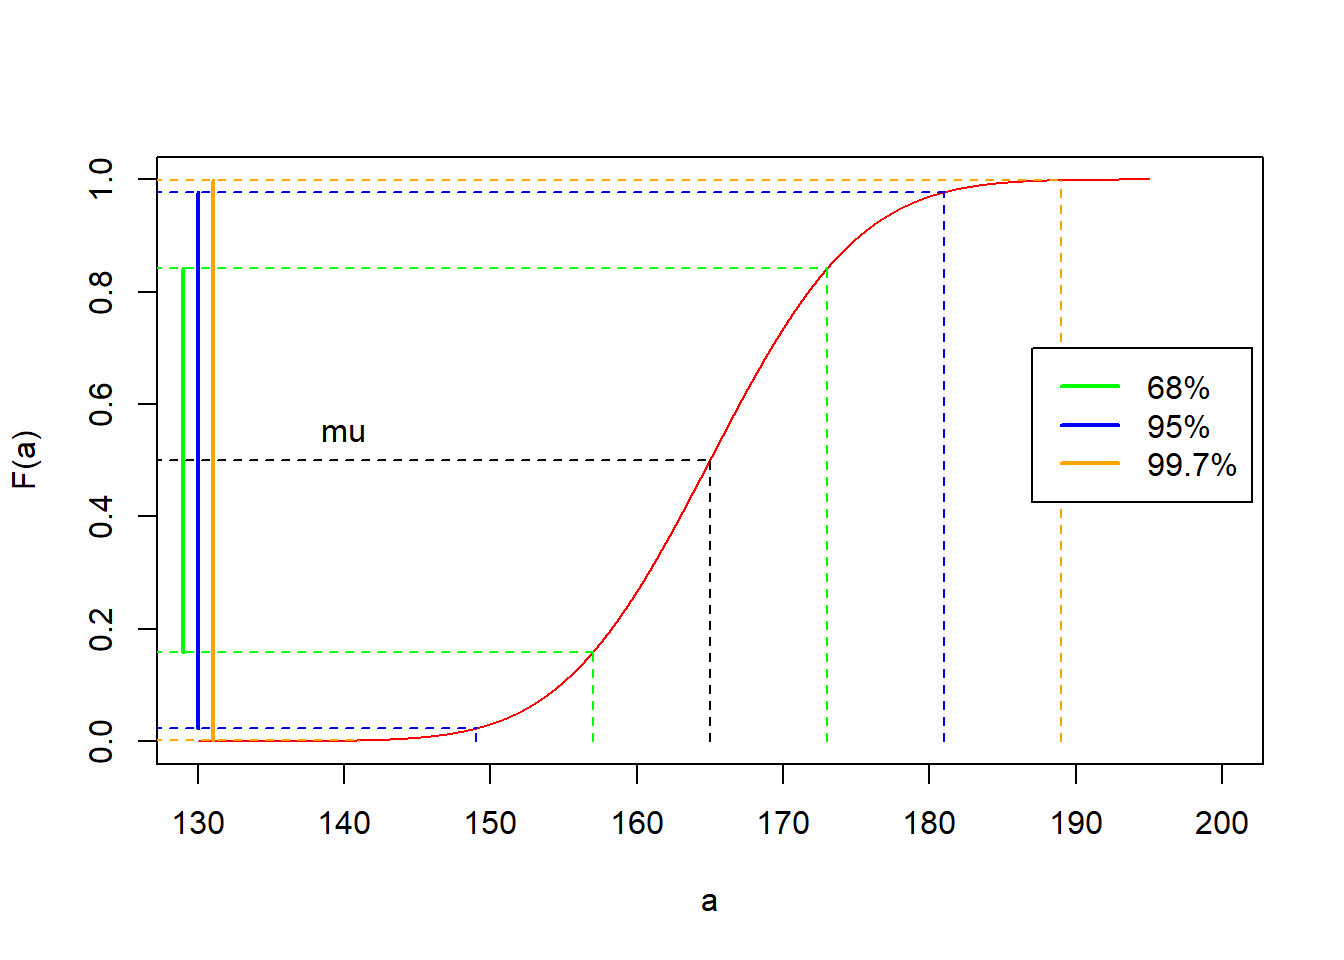
\includegraphics{_main_files/figure-latex/unnamed-chunk-3-1.pdf}

\begin{center}\rule{0.5\linewidth}{0.5pt}\end{center}

\begin{center}\rule{0.5\linewidth}{0.5pt}\end{center}

\hypertarget{gruxe1fico-de-sectores}{%
\section{Gráfico de sectores}\label{gruxe1fico-de-sectores}}

Podemos visualizar las frecuencias relativas con un gráfico de sectores

\begin{itemize}
\tightlist
\item
  Donde el área del círculo representa el 100\% de las observaciones (proporción = 1) y las secciones las frecuencias relativas de todos los resultados.
\end{itemize}

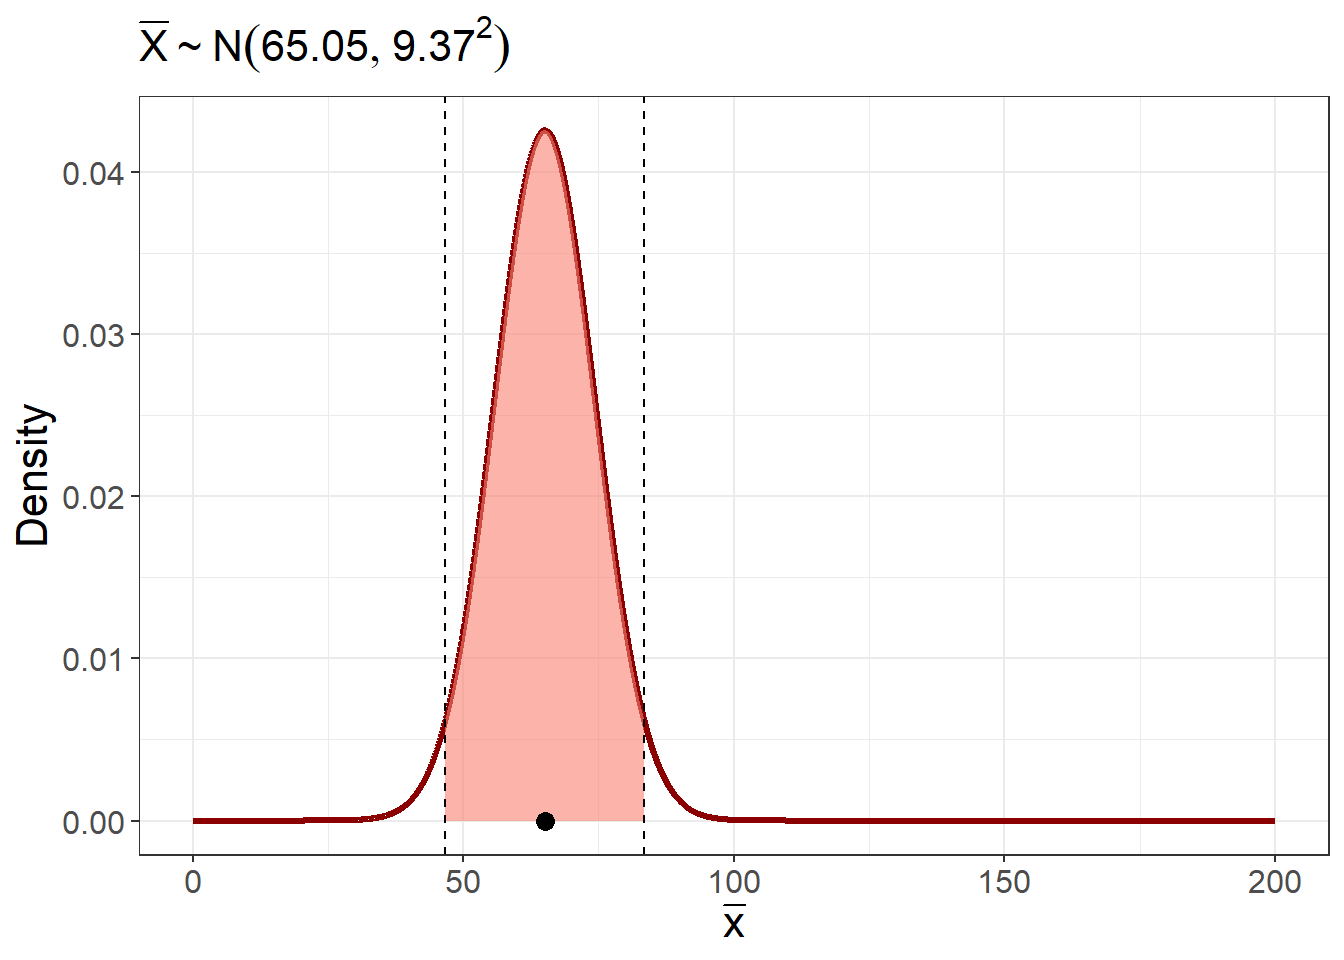
\includegraphics{_main_files/figure-latex/unnamed-chunk-4-1.pdf}

\begin{center}\rule{0.5\linewidth}{0.5pt}\end{center}

\begin{center}\rule{0.5\linewidth}{0.5pt}\end{center}

\hypertarget{variables-categuxf3ricas-y-ordenadas}{%
\section{Variables categóricas y ordenadas}\label{variables-categuxf3ricas-y-ordenadas}}

Los tipos de células no están ordenados de manera lógica en relación con los resultados. Sin embargo, a veces las variables \textbf{categóricas} se pueden \textbf{ordenar}.

Estudio de misofonía:

\begin{itemize}
\item
  123 pacientes fueron examinados por misofonía: ansiedad/ira producida por ciertos sonidos
\item
  Se clasificaron en 4 grupos diferentes según la gravedad.
\end{itemize}

\begin{center}\rule{0.5\linewidth}{0.5pt}\end{center}

\begin{center}\rule{0.5\linewidth}{0.5pt}\end{center}

\hypertarget{ejemplo-2}{%
\section{Ejemplo}\label{ejemplo-2}}

Los resultados del estudio son:

\begin{verbatim}
##   [1] 4 2 0 3 0 0 2 3 0 3 0 2 2 0 2 0 0 3 3 0 3 3 2 0 0 0 4 2 2 0 2 0 0 0 3 0 2
##  [38] 3 2 2 0 2 3 0 0 2 2 3 3 0 0 4 3 3 2 0 2 0 0 0 2 2 0 0 2 3 0 1 3 2 4 3 2 3
##  [75] 0 2 3 2 4 1 2 0 2 0 2 0 2 2 4 3 0 3 0 0 0 2 2 1 3 0 0 3 2 1 3 0 4 4 2 3 3
## [112] 3 0 3 2 1 2 3 3 4 2 3 2
\end{verbatim}

y su tabla de frecuencias

\begin{verbatim}
##   outcome ni         fi
## 1       0 41 0.33333333
## 2       1  5 0.04065041
## 3       2 37 0.30081301
## 4       3 31 0.25203252
## 5       4  9 0.07317073
\end{verbatim}

\begin{center}\rule{0.5\linewidth}{0.5pt}\end{center}

\begin{center}\rule{0.5\linewidth}{0.5pt}\end{center}

\hypertarget{frecuencias-acumuladas-absolutas-y-relativas}{%
\section{Frecuencias acumuladas absolutas y relativas}\label{frecuencias-acumuladas-absolutas-y-relativas}}

La gravedad de la misofonía es \textbf{categórica} y \textbf{ordenada}.

Cuando los resultados se pueden ordenar, entonces es útil preguntarse por el \textbf{número} de observaciones que se obtuvieron hasta un resultado dado. Llamamos a este número la frecuencia acumulada absoluta hasta el resultado \(i\):
\[N_i=\sum_{k=1..i} n_k\]

Tambíen es útil calcular la \textbf{proporción} de las observaciones que se obtuvo hasta un resultado dado

\[F_i=\sum_{k=1..i} f_k\]

\begin{center}\rule{0.5\linewidth}{0.5pt}\end{center}

\begin{center}\rule{0.5\linewidth}{0.5pt}\end{center}

\hypertarget{tabla-de-frecuencia} de los pacientes tenían misofonía hasta la gravedad \textbf{2}
\item
  \textbf{37\%} de los pacientes tienen una gravedad menor o igual a \textbf{1}
\end{itemize}

\begin{center}\rule{0.5\linewidth}{0.5pt}\end{center}

\begin{center}\rule{0.5\linewidth}{0.5pt}\end{center}

\hypertarget{gruxe1fica-de-frecuencia-acumulada}{%
\section{Gráfica de frecuencia acumulada}\label{gruxe1fica-de-frecuencia-acumulada}}

También podemos graficar la frecuencia acumulada Vs los resultados

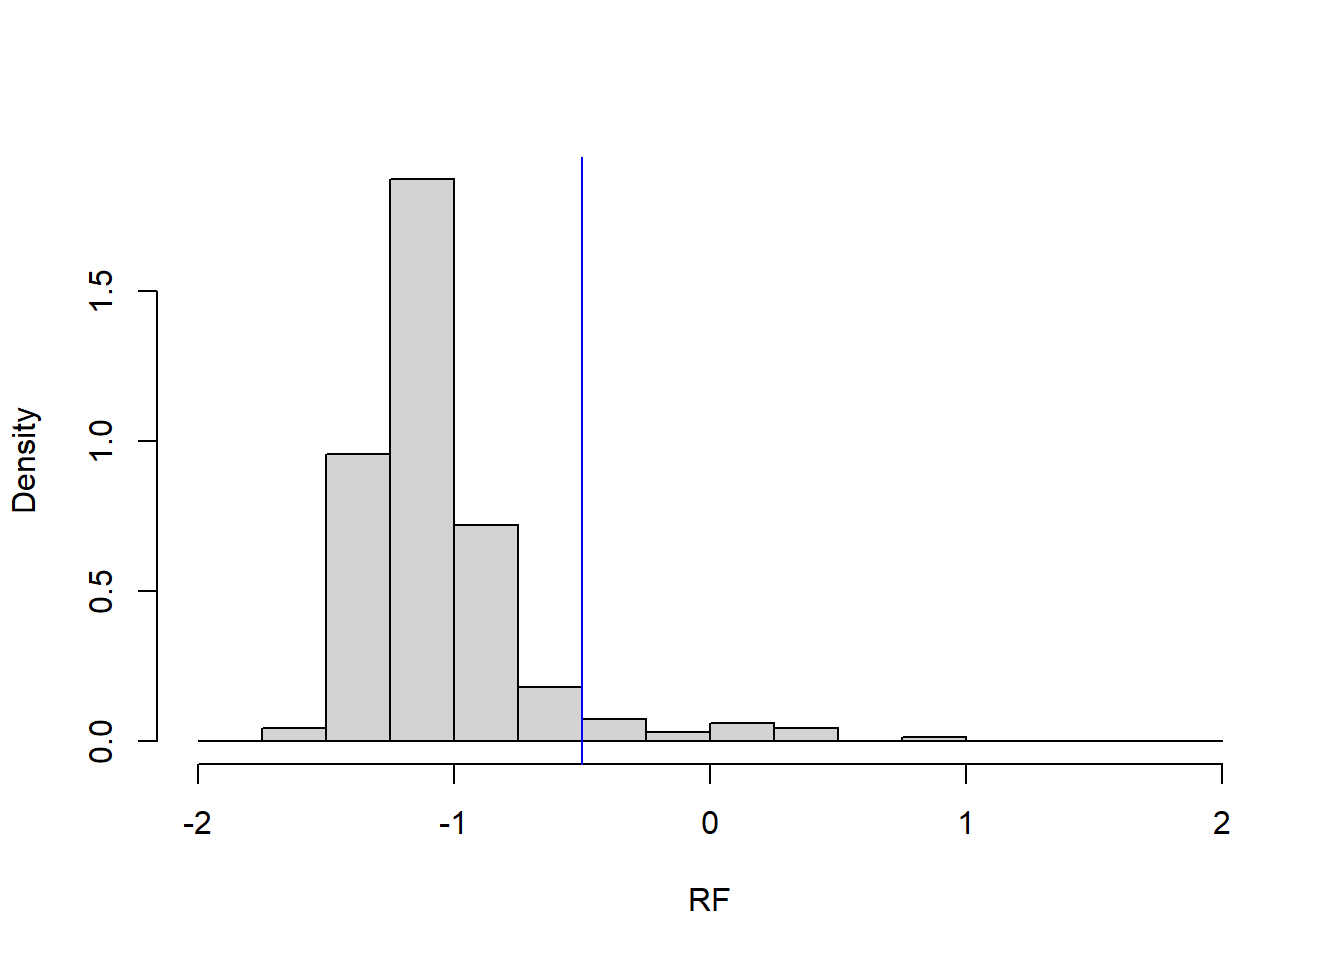
\includegraphics{_main_files/figure-latex/unnamed-chunk-8-1.pdf}
\_\_\_\_\_\_\_\_\_\_\_
\_\_\_\_\_\_\_\_\_\_\_

\hypertarget{variables-continuas}{%
\section{Variables continuas}\label{variables-continuas}}

El resultado de un experimento aleatorio también puede dar resultados continuos.

En el estudio de misofonía, los investigadores se preguntaron si la convexidad de la mandíbula afectaría la gravedad de la misofonía (la hipótesis científica es que el ángulo de convexidad de la mandíbula puede influir en el oído y su sensibilidad). Estos son los resultados para la convexidad de la mandíbula (grados)

\begin{verbatim}
##   [1]  7.97 18.23 12.27  7.81  9.81 13.50 19.30  7.70 12.30  7.90 12.60 19.00
##  [13]  7.27 14.00  5.40  8.00 11.20  7.75  7.94 16.69  7.62  7.02  7.00 19.20
##  [25]  7.96 14.70  7.24  7.80  7.90  4.70  4.40 14.00 14.40 16.00  1.40  9.76
##  [37]  7.90  7.90  7.40  6.30  7.76  7.30  7.00 11.23 16.00  7.90  7.29  6.91
##  [49]  7.10 13.40 11.60 -1.00  6.00  7.82  4.80 11.00  9.00 11.50 16.00 15.00
##  [61]  1.40 16.80  7.70 16.14  7.12 -1.00 17.00  9.26 18.70  3.40 21.30  7.50
##  [73]  6.03  7.50 19.00 19.01  8.10  7.80  6.10 15.26  7.95 18.00  4.60 15.00
##  [85]  7.50  8.00 16.80  8.54  7.00 18.30  7.80 16.00 14.00 12.30 11.40  8.50
##  [97]  7.00  7.96 17.60 10.00  3.50  6.70 17.00 20.26  6.64  1.80  7.02  2.46
## [109] 19.00 17.86  6.10  6.64 12.00  6.60  8.70 14.05  7.20 19.70  7.70  6.02
## [121]  2.50 19.00  6.80
\end{verbatim}

\begin{center}\rule{0.5\linewidth}{0.5pt}\end{center}

\begin{center}\rule{0.5\linewidth}{0.5pt}\end{center}

\hypertarget{contenedores}{%
\section{Contenedores}\label{contenedores}}

¡Los resultados continuos no se pueden contar!

Las transformamos en variables categóricas ordenadas

\begin{itemize}
\tightlist
\item
  Cubrimos el rango de las observaciones en intervalos regulares del mismo tamaño (bins)
\end{itemize}

\begin{verbatim}
## [1] "[-1.02,3.46]" "(3.46,7.92]"  "(7.92,12.4]"  "(12.4,16.8]"  "(16.8,21.3]"
\end{verbatim}

\begin{center}\rule{0.5\linewidth}{0.5pt}\end{center}

\begin{center}\rule{0.5\linewidth}{0.5pt}\end{center}

\hypertarget{crear-una-variable-categuxf3rica-a-partir-de-una-continua}{%
\section{Crear una variable categórica a partir de una continua}\label{crear-una-variable-categuxf3rica-a-partir-de-una-continua}}

\begin{itemize}
\tightlist
\item
  Asignamos cada observación a su intervalo: creando una variable categórica \textbf{ordenada}; en este caso con 5 resultados posibles
\end{itemize}

\begin{verbatim}
##   [1] "(7.92,12.4]"  "(16.8,21.3]"  "(7.92,12.4]"  "(3.46,7.92]"  "(7.92,12.4]" 
##   [6] "(12.4,16.8]"  "(16.8,21.3]"  "(3.46,7.92]"  "(7.92,12.4]"  "(3.46,7.92]" 
##  [11] "(12.4,16.8]"  "(16.8,21.3]"  "(3.46,7.92]"  "(12.4,16.8]"  "(3.46,7.92]" 
##  [16] "(7.92,12.4]"  "(7.92,12.4]"  "(3.46,7.92]"  "(7.92,12.4]"  "(12.4,16.8]" 
##  [21] "(3.46,7.92]"  "(3.46,7.92]"  "(3.46,7.92]"  "(16.8,21.3]"  "(7.92,12.4]" 
##  [26] "(12.4,16.8]"  "(3.46,7.92]"  "(3.46,7.92]"  "(3.46,7.92]"  "(3.46,7.92]" 
##  [31] "(3.46,7.92]"  "(12.4,16.8]"  "(12.4,16.8]"  "(12.4,16.8]"  "[-1.02,3.46]"
##  [36] "(7.92,12.4]"  "(3.46,7.92]"  "(3.46,7.92]"  "(3.46,7.92]"  "(3.46,7.92]" 
##  [41] "(3.46,7.92]"  "(3.46,7.92]"  "(3.46,7.92]"  "(7.92,12.4]"  "(12.4,16.8]" 
##  [46] "(3.46,7.92]"  "(3.46,7.92]"  "(3.46,7.92]"  "(3.46,7.92]"  "(12.4,16.8]" 
##  [51] "(7.92,12.4]"  "[-1.02,3.46]" "(3.46,7.92]"  "(3.46,7.92]"  "(3.46,7.92]" 
##  [56] "(7.92,12.4]"  "(7.92,12.4]"  "(7.92,12.4]"  "(12.4,16.8]"  "(12.4,16.8]" 
##  [61] "[-1.02,3.46]" "(12.4,16.8]"  "(3.46,7.92]"  "(12.4,16.8]"  "(3.46,7.92]" 
##  [66] "[-1.02,3.46]" "(16.8,21.3]"  "(7.92,12.4]"  "(16.8,21.3]"  "[-1.02,3.46]"
##  [71] "(16.8,21.3]"  "(3.46,7.92]"  "(3.46,7.92]"  "(3.46,7.92]"  "(16.8,21.3]" 
##  [76] "(16.8,21.3]"  "(7.92,12.4]"  "(3.46,7.92]"  "(3.46,7.92]"  "(12.4,16.8]" 
##  [81] "(7.92,12.4]"  "(16.8,21.3]"  "(3.46,7.92]"  "(12.4,16.8]"  "(3.46,7.92]" 
##  [86] "(7.92,12.4]"  "(12.4,16.8]"  "(7.92,12.4]"  "(3.46,7.92]"  "(16.8,21.3]" 
##  [91] "(3.46,7.92]"  "(12.4,16.8]"  "(12.4,16.8]"  "(7.92,12.4]"  "(7.92,12.4]" 
##  [96] "(7.92,12.4]"  "(3.46,7.92]"  "(7.92,12.4]"  "(16.8,21.3]"  "(7.92,12.4]" 
## [101] "(3.46,7.92]"  "(3.46,7.92]"  "(16.8,21.3]"  "(16.8,21.3]"  "(3.46,7.92]" 
## [106] "[-1.02,3.46]" "(3.46,7.92]"  "[-1.02,3.46]" "(16.8,21.3]"  "(16.8,21.3]" 
## [111] "(3.46,7.92]"  "(3.46,7.92]"  "(7.92,12.4]"  "(3.46,7.92]"  "(7.92,12.4]" 
## [116] "(12.4,16.8]"  "(3.46,7.92]"  "(16.8,21.3]"  "(3.46,7.92]"  "(3.46,7.92]" 
## [121] "[-1.02,3.46]" "(16.8,21.3]"  "(3.46,7.92]"
\end{verbatim}

\begin{center}\rule{0.5\linewidth}{0.5pt}\end{center}

\begin{center}\rule{0.5\linewidth}{0.5pt}\end{center}

\hypertarget{tabla-de-frecuencias-para-una-variable-continua}{%
\section{Tabla de frecuencias para una variable continua}\label{tabla-de-frecuencias-para-una-variable-continua}}

\begin{verbatim}
##        outcome ni         fi  Ni         Fi
## 1 [-1.02,3.46]  8 0.06504065   8 0.06504065
## 2  (3.46,7.92] 51 0.41463415  59 0.47967480
## 3  (7.92,12.4] 26 0.21138211  85 0.69105691
## 4  (12.4,16.8] 20 0.16260163 105 0.85365854
## 5  (16.8,21.3] 18 0.14634146 123 1.00000000
\end{verbatim}

\begin{center}\rule{0.5\linewidth}{0.5pt}\end{center}

\begin{center}\rule{0.5\linewidth}{0.5pt}\end{center}

\hypertarget{histograma}{%
\section{Histograma}\label{histograma}}

El histograma es la gráfica de \(n_i\) o \(f_i\) Vs los resultados (bins). El histograma depende del tamaño de los contenedores.

\begin{center}\rule{0.5\linewidth}{0.5pt}\end{center}

\begin{center}\rule{0.5\linewidth}{0.5pt}\end{center}

\hypertarget{tabla-de-frecuencias-para-una-variable-continua-1}{%
\section{Tabla de frecuencias para una variable continua}\label{tabla-de-frecuencias-para-una-variable-continua-1}}

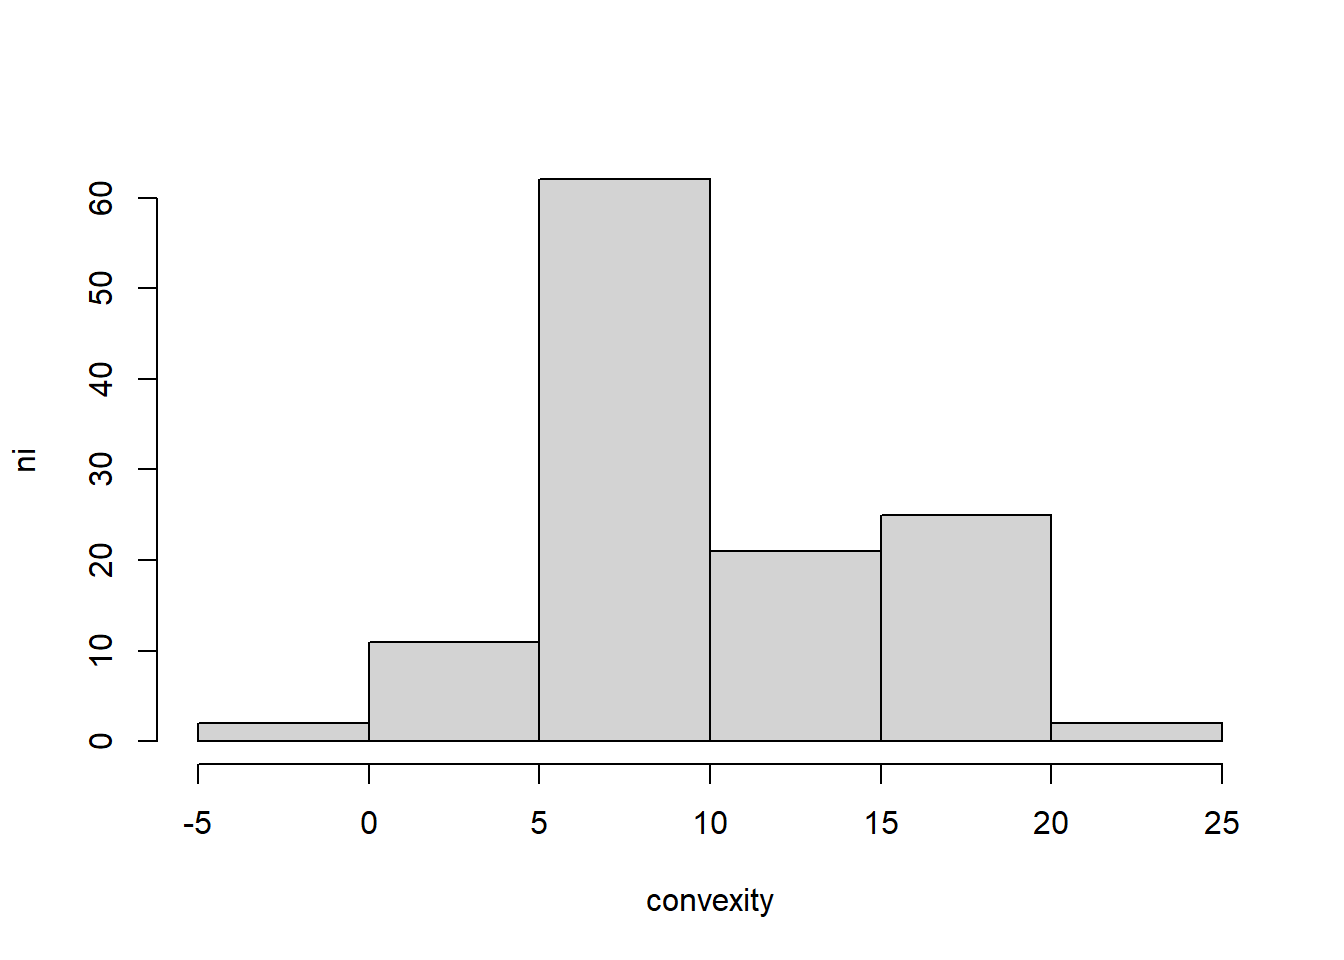
\includegraphics{_main_files/figure-latex/unnamed-chunk-13-1.pdf}

\begin{center}\rule{0.5\linewidth}{0.5pt}\end{center}

\begin{center}\rule{0.5\linewidth}{0.5pt}\end{center}

\hypertarget{histograma-1}{%
\section{Histograma}\label{histograma-1}}

El histograma es la gráfica de \(n_i\) o \(f_i\) Vs los resultados (bins). El histograma depende del tamaño de los contenedores.

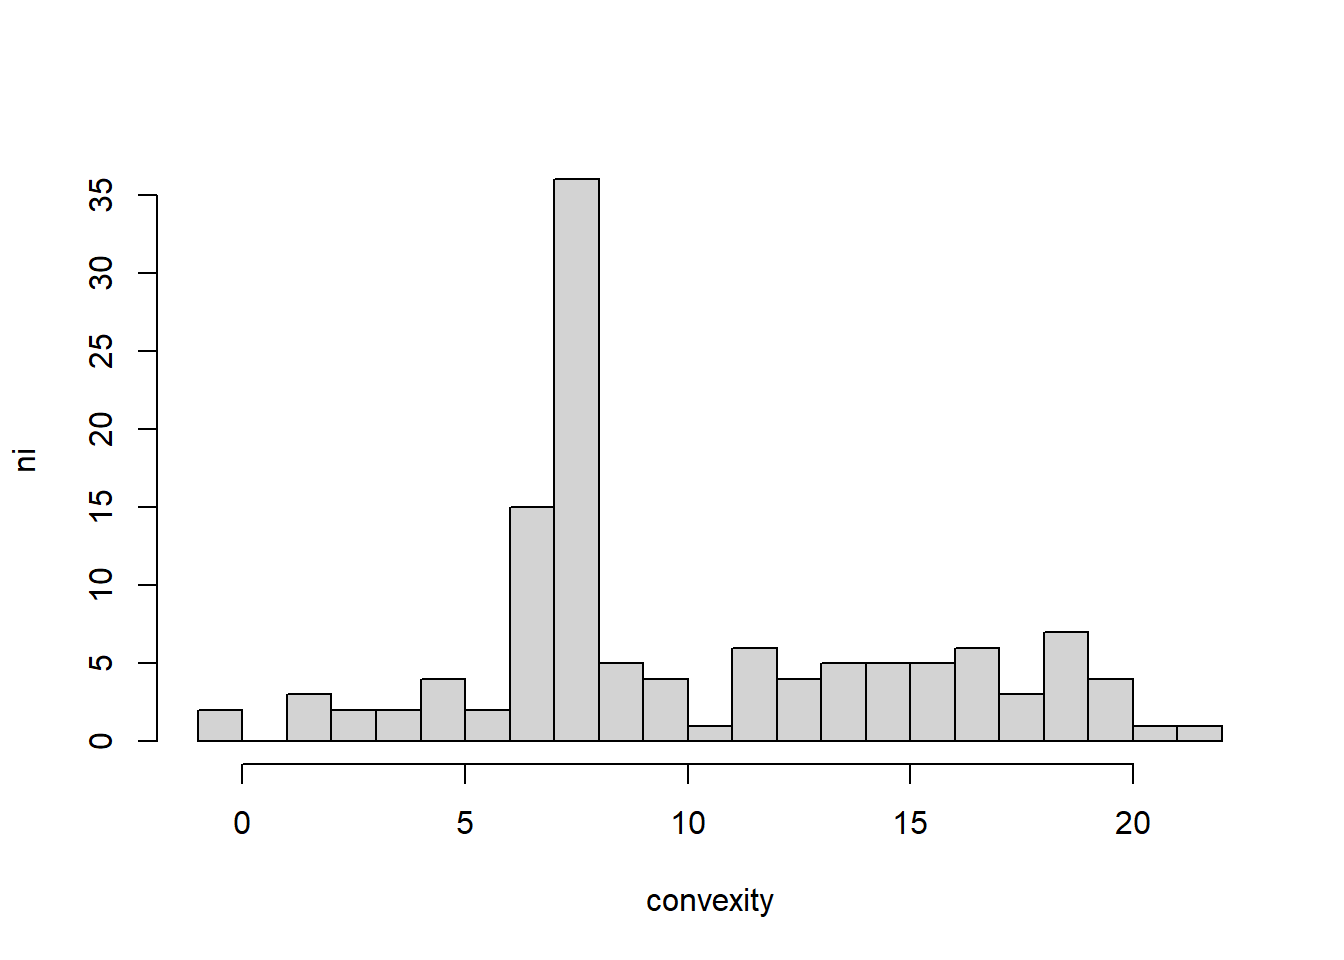
\includegraphics{_main_files/figure-latex/unnamed-chunk-14-1.pdf}

\begin{center}\rule{0.5\linewidth}{0.5pt}\end{center}

\begin{center}\rule{0.5\linewidth}{0.5pt}\end{center}

\hypertarget{gruxe1fica-de-frecuencia-acumulada-variables-continuas}{%
\section{Gráfica de frecuencia acumulada: Variables continuas}\label{gruxe1fica-de-frecuencia-acumulada-variables-continuas}}

También podemos graficar la frecuencia acumulada Vs los resultados

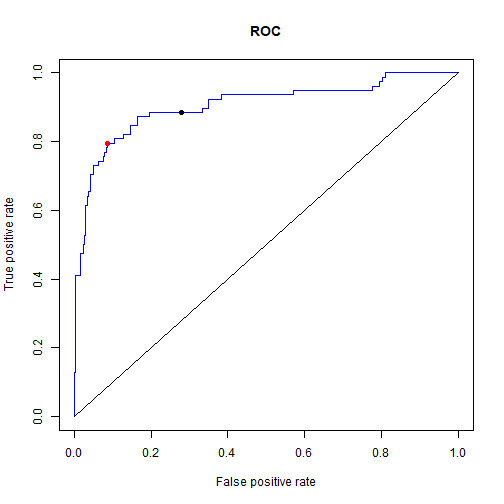
\includegraphics{_main_files/figure-latex/unnamed-chunk-15-1.pdf}

\begin{center}\rule{0.5\linewidth}{0.5pt}\end{center}

\begin{center}\rule{0.5\linewidth}{0.5pt}\end{center}

\hypertarget{resumen-estaduxedstico}{%
\section{Resumen estadístico}\label{resumen-estaduxedstico}}

Las estadísticas de resumen son números calculados a partir de los datos que nos dicen características importantes de las variables numéricas (categóricas o continuas).

Valores límite:

\begin{itemize}
\tightlist
\item
  mínimo: el resultado mínimo observado
\item
  máximo: el resultado máximo observado
\end{itemize}

Valor central para los resultados

\begin{itemize}
\tightlist
\item
  El promedio se define como
\end{itemize}

\[\bar{x}=\frac{1}{N} \sum_{j=1..N} x_j\]

donde \(x_j\) es la \textbf{observación} \(j\) (convexidad) de un total de \(N\).

\begin{center}\rule{0.5\linewidth}{0.5pt}\end{center}

\begin{center}\rule{0.5\linewidth}{0.5pt}\end{center}

\hypertarget{promedio}{%
\section{Promedio}\label{promedio}}

La convexidad promedio se puede calcular directamente a partir de las \textbf{observaciones}

\(\bar{x}= \frac{1}{N}\sum_j x_j\)

\(= \frac{1}{N}(7.97 + 18.23 + 12.27... + 6.80) = 10.19894\)

\begin{center}\rule{0.5\linewidth}{0.5pt}\end{center}

\begin{center}\rule{0.5\linewidth}{0.5pt}\end{center}

\hypertarget{promedio-ordenado-categuxf3ricamente}{%
\section{Promedio (ordenado categóricamente)}\label{promedio-ordenado-categuxf3ricamente}}

Para las variables \textbf{ordenadas categóricamente}, podemos usar la tabla de frecuencias para calcular el promedio

\begin{verbatim}
##   outcome ni         fi
## 1       0 41 0.33333333
## 2       1  5 0.04065041
## 3       2 37 0.30081301
## 4       3 31 0.25203252
## 5       4  9 0.07317073
\end{verbatim}

La \textbf{severidad} promedio de la misofonía en el estudio
\textbf{también} puede calcularse a partir de las frecuencias relativas de los \textbf{resultados}

\(\bar{x}=\frac{1}{N}\sum_{i=1...N} x_j=\frac{1}{N}\sum_{i=1...M} x_i*n_ {i}=\sum_{i=1...M} x_i*f_{i}\)

\(=0*f_{0}+1*f_{1}+2*f_{2}+3*f_{3}+4*f_{4}=1,691057\)

(note el cambio de \(N\) a \(M\) en la segunda suma)

\begin{center}\rule{0.5\linewidth}{0.5pt}\end{center}

\begin{center}\rule{0.5\linewidth}{0.5pt}\end{center}

\hypertarget{promedio-ordenado-categuxf3ricamente-1}{%
\section{Promedio (ordenado categóricamente)}\label{promedio-ordenado-categuxf3ricamente-1}}

En términos de los \textbf{resultados} de las variables ordenadas categóricas, el \textbf{promedio} se puede escribir como

\[\bar{x}= \sum_{i = 1...M} x_i f_i\]

de un total de \(M\) posibles resultados (número de niveles de gravedad).

\(\bar{x}\) es el \textbf{valor central} o centro de gravedad de los resultados. Como si cada resultado tuviera una densidad de masa dada por \(f_i\).

\begin{center}\rule{0.5\linewidth}{0.5pt}\end{center}

\begin{center}\rule{0.5\linewidth}{0.5pt}\end{center}

\hypertarget{promedio-1}{%
\section{Promedio}\label{promedio-1}}

\begin{itemize}
\item
  El promedio no es el resultado de una observación (experimento aleatorio).
\item
  Es el resultado de una serie de observaciones (muestra).
\item
  Describe el número donde se equilibran los valores observados.
\end{itemize}

Por eso escuchamos, por ejemplo, que un paciente con una infección puede contagiar a una media de 2,5 personas.

\begin{center}\rule{0.5\linewidth}{0.5pt}\end{center}

\begin{center}\rule{0.5\linewidth}{0.5pt}\end{center}

\hypertarget{promedio-2}{%
\section{Promedio}\label{promedio-2}}

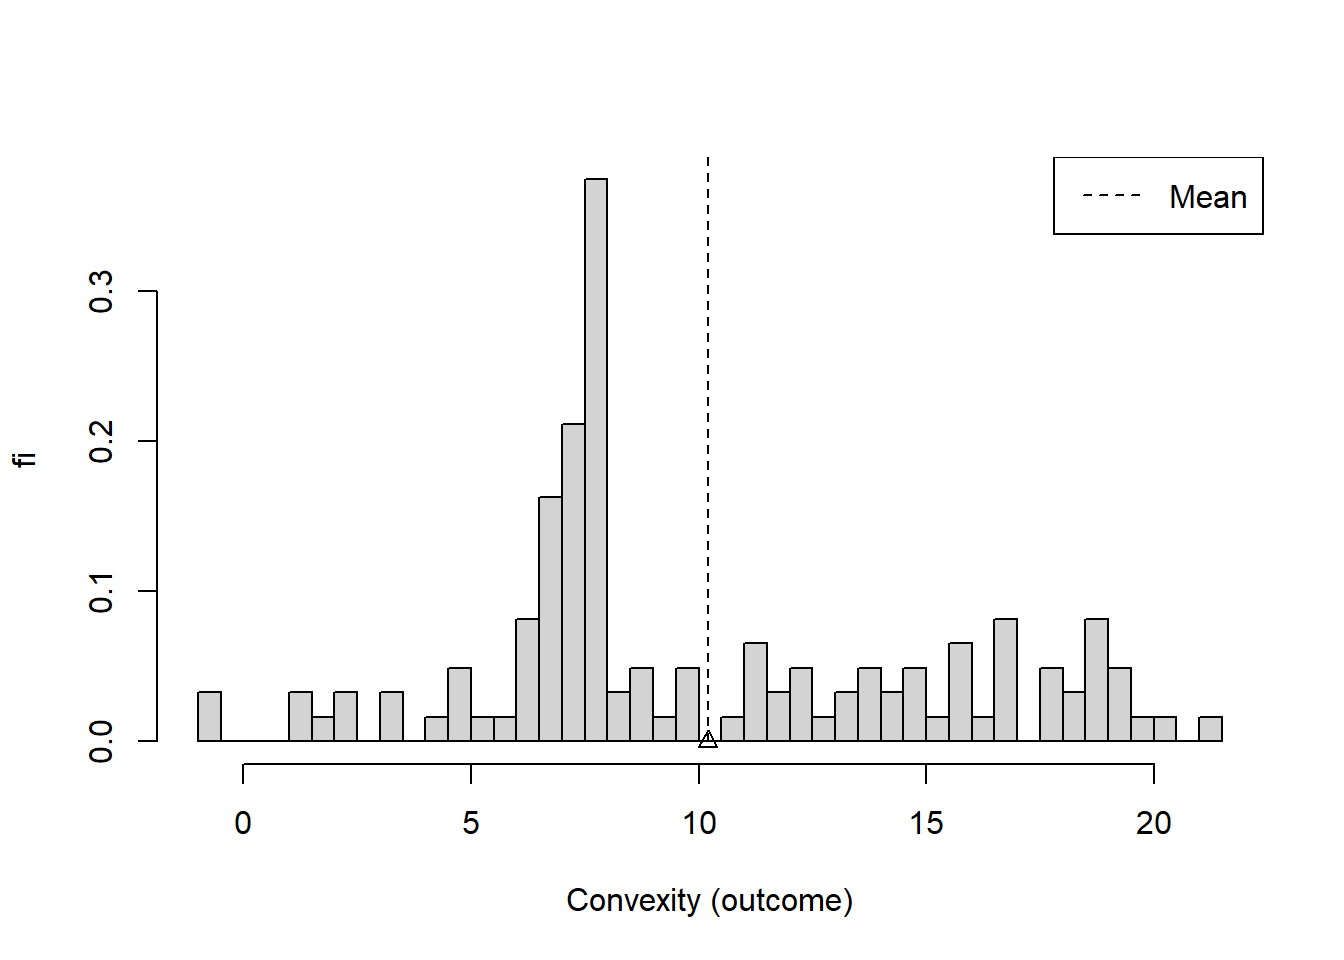
\includegraphics{_main_files/figure-latex/unnamed-chunk-17-1.pdf}

\begin{center}\rule{0.5\linewidth}{0.5pt}\end{center}

\begin{center}\rule{0.5\linewidth}{0.5pt}\end{center}

\hypertarget{mediana}{%
\section{mediana}\label{mediana}}

Otra medida de centralidad es la mediana. La mediana \(q_{0.5}\) es el valor \(x_p\)

\[mediana(x)=q_{0.5}=x_p\]

debajo del cual encontramos la mitad de las observaciones

\[\sum_{x\leq x_p} 1 = \frac{N}{2}\]

o en términos de frecuencias, es el valor \(x_p\) que hace que la frecuencia acumulada \(F_p\) sea igual a \(0.5\)

\[q_{0.5}=\sum_{x\leq x_p} f_x =F_p=0.5\]

\begin{center}\rule{0.5\linewidth}{0.5pt}\end{center}

\begin{center}\rule{0.5\linewidth}{0.5pt}\end{center}

\hypertarget{mediana-vs-promedio}{%
\section{Mediana Vs Promedio}\label{mediana-vs-promedio}}

\begin{itemize}
\tightlist
\item
  Promedio: Centro de masa (compensa valores distantes)
\item
  Mediana: La mitad de la masa
\end{itemize}

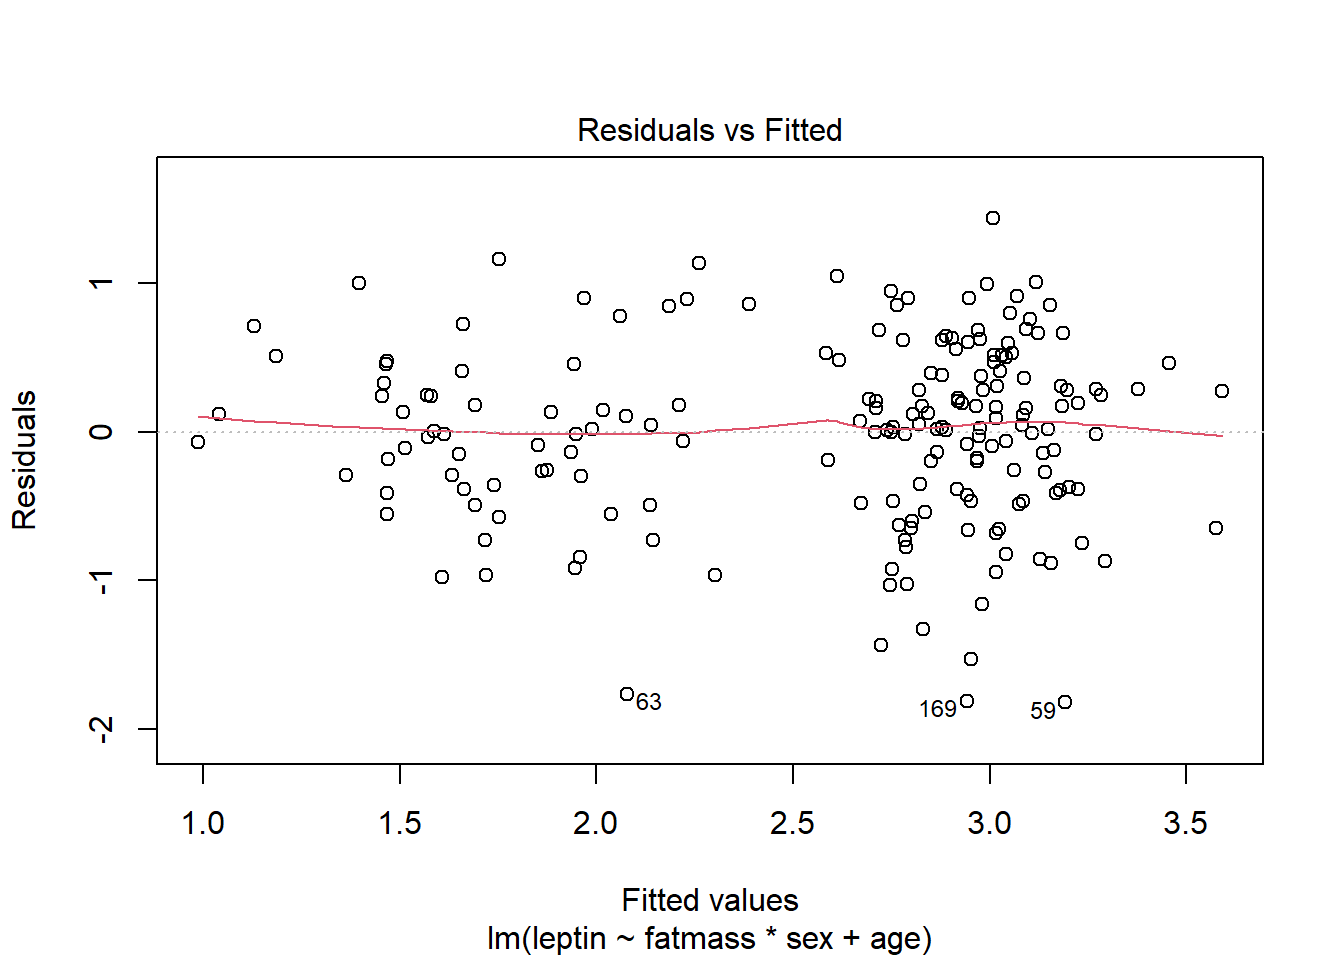
\includegraphics{_main_files/figure-latex/unnamed-chunk-18-1.pdf}

\begin{center}\rule{0.5\linewidth}{0.5pt}\end{center}

\begin{center}\rule{0.5\linewidth}{0.5pt}\end{center}

\hypertarget{dispersiuxf3n}{%
\section{Dispersión}\label{dispersiuxf3n}}

Una medida importante de los resultados es su \textbf{dispersión}. Muchos experimentos pueden compartir su media, pero difieren en la dispersión de los valores.

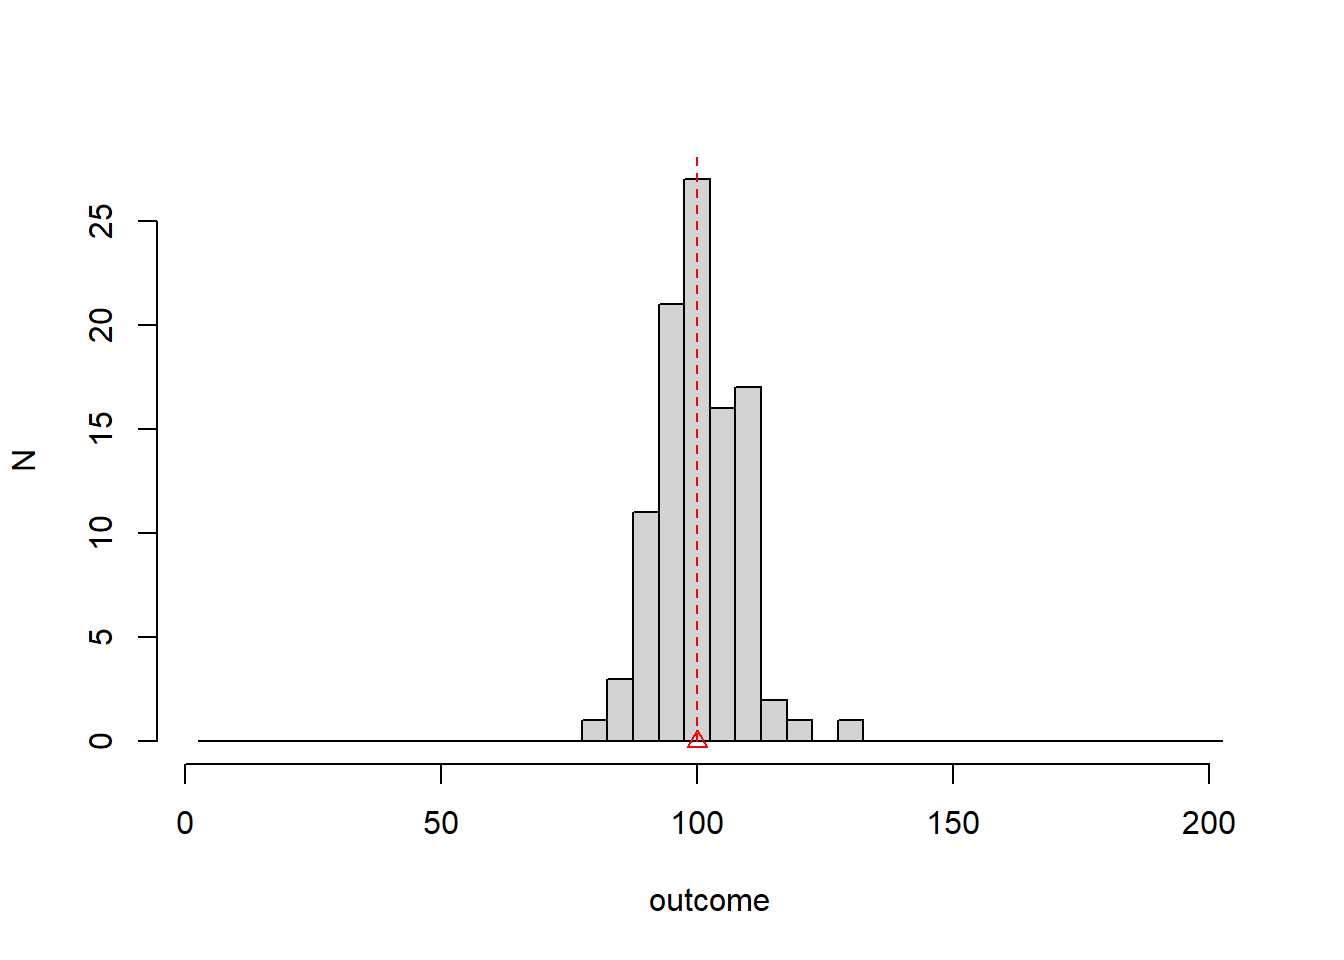
\includegraphics{_main_files/figure-latex/unnamed-chunk-19-1.pdf}

\begin{center}\rule{0.5\linewidth}{0.5pt}\end{center}

\begin{center}\rule{0.5\linewidth}{0.5pt}\end{center}

\hypertarget{dispersiuxf3n-1}{%
\section{Dispersión}\label{dispersiuxf3n-1}}

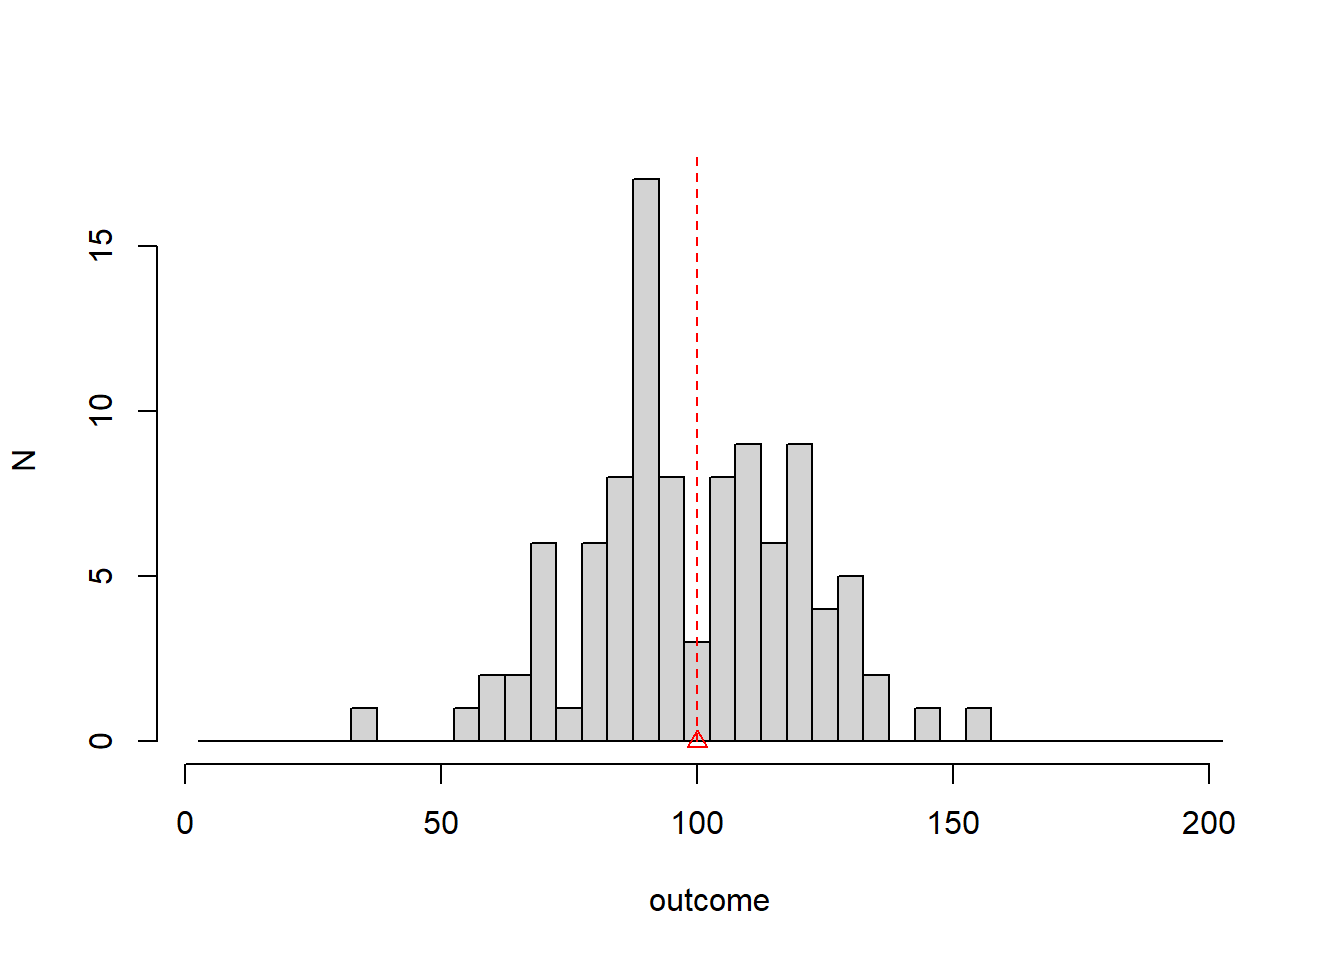
\includegraphics{_main_files/figure-latex/unnamed-chunk-20-1.pdf}

\begin{center}\rule{0.5\linewidth}{0.5pt}\end{center}

\begin{center}\rule{0.5\linewidth}{0.5pt}\end{center}

\hypertarget{variaciuxf3n-de-la-muestra}{%
\section{Variación de la muestra}\label{variaciuxf3n-de-la-muestra}}

La dispersión con respecto a la media se mide con el

\begin{itemize}
\tightlist
\item
  La varianza muestral:
\end{itemize}

\[s^2=\frac{1}{N-1} \sum_{j=1..N} (x_j-\bar{x})^2\]

Mide la distancia cuadrada promedio de las \textbf{observaciones} al promedio. La razón de \(N-1\) se explicará cuando hablemos de inferencia.

\begin{center}\rule{0.5\linewidth}{0.5pt}\end{center}

\begin{center}\rule{0.5\linewidth}{0.5pt}\end{center}

\hypertarget{variaciuxf3n-de-la-muestra-1}{%
\section{Variación de la muestra}\label{variaciuxf3n-de-la-muestra-1}}

\begin{itemize}
\tightlist
\item
  En términos de frecuencias de variables \textbf{categóricas y ordenadas}
\end{itemize}

\[s^2=\frac{N}{N-1} \sum_{x} (x-\bar{x})^2 f_x\]

\(s^2\) se puede considerar como el momento de inercia de las observaciones.

\begin{center}\rule{0.5\linewidth}{0.5pt}\end{center}

\begin{center}\rule{0.5\linewidth}{0.5pt}\end{center}

\hypertarget{desviaciuxf3n-estuxe1ndar}{%
\section{Desviación Estándar}\label{desviaciuxf3n-estuxe1ndar}}

La raíz cuadrada de la varianza de la muestra se denomina \textbf{desviación estándar} \(s\).

La desviación estándar del ángulo de convexidad es

\(s= [\frac{1}{123-1}((7,97-10,19894)^2+ (18,23-10,19894)^2\)
\(+ (12,27-10,19894)^2 + ...)]^{1/2} = 5,086707\)

La convexidad de la mandíbula se desvía de su media en \(5,086707\).

\begin{center}\rule{0.5\linewidth}{0.5pt}\end{center}

\begin{center}\rule{0.5\linewidth}{0.5pt}\end{center}

\hypertarget{ric}{%
\section{RIC}\label{ric}}

\begin{itemize}
\item
  La dispersión de datos también se puede medir con respecto a la mediana por el \textbf{rango intercuartílico}
\item
  Definimos el \textbf{primer} cuartil como el valor \(x_p\) que hace que la frecuencia acumulada \(F_p\) sea igual a \(0,25\)
\end{itemize}

\[q_{0.25}=\sum_{x\leq x_p} f_x =F_p=0.25\]

\begin{itemize}
\tightlist
\item
  También definimos el \textbf{tercer} cuartil como el valor \(x_p\) que hace que la frecuencia acumulada \(F_p\) sea igual a \(0,75\)
\end{itemize}

\[q_{0.75}=\sum_{x\leq x_p} f_x =F_p=0.75\]

\begin{center}\rule{0.5\linewidth}{0.5pt}\end{center}

\begin{center}\rule{0.5\linewidth}{0.5pt}\end{center}

\hypertarget{ric-1}{%
\section{RIC}\label{ric-1}}

La distancia entre el tercer cuartil y el primer cuartil se denomina \textbf{rango intercuartílico} (RIC) y captura el 50 \% central de las observaciones

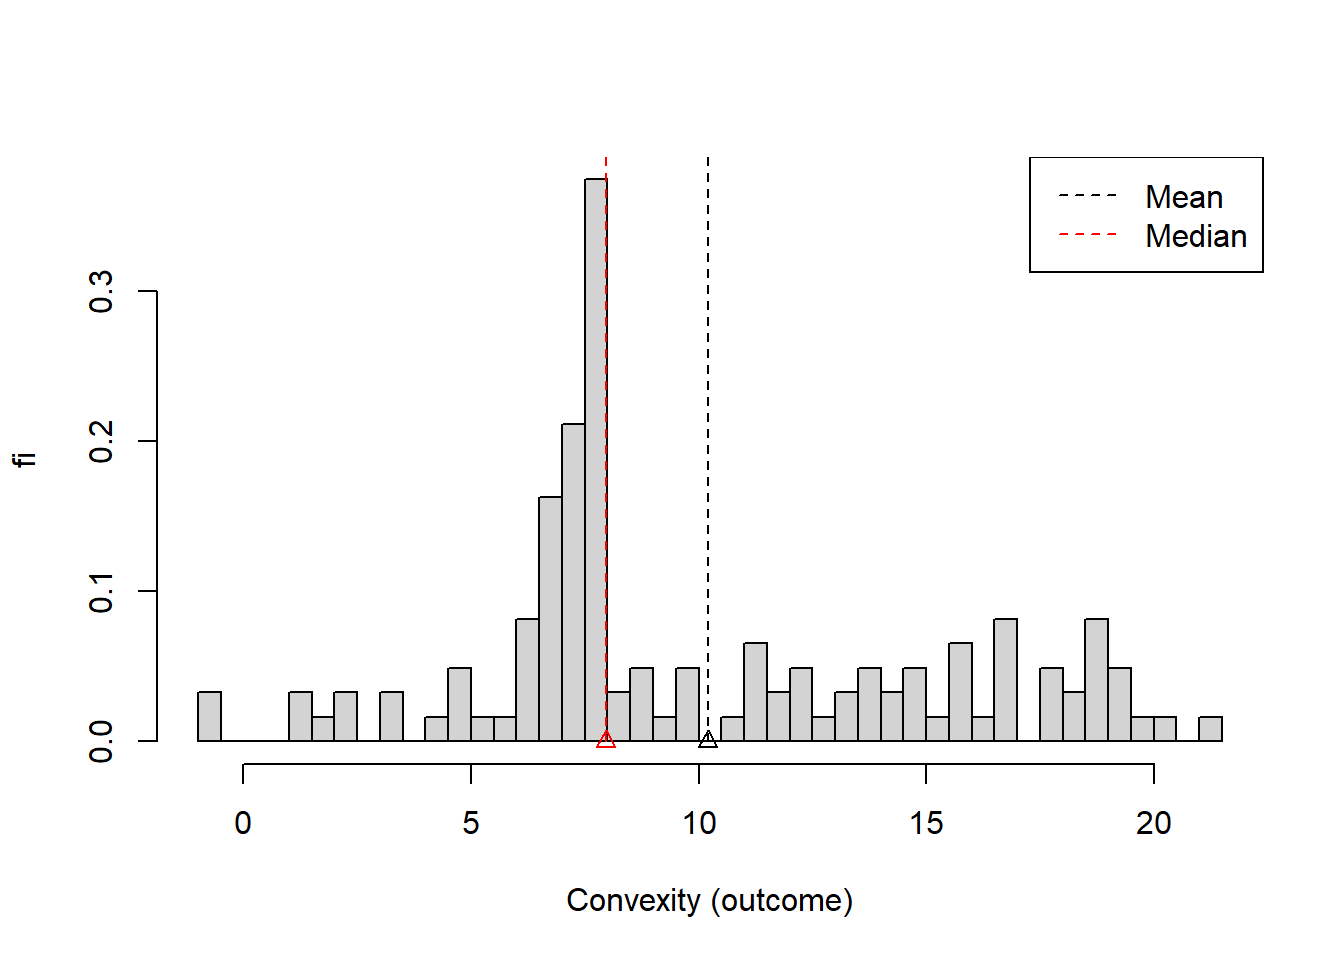
\includegraphics{_main_files/figure-latex/unnamed-chunk-21-1.pdf}

\begin{center}\rule{0.5\linewidth}{0.5pt}\end{center}

\begin{center}\rule{0.5\linewidth}{0.5pt}\end{center}

\hypertarget{diagrama-de-caja}{%
\section{Diagrama de caja}\label{diagrama-de-caja}}

El rango intercuartílico, la mediana y el 5 \% y el 95 \% de los datos se pueden visualizar en un \textbf{diagrama de caja}, aquí los valores de los resultados están en el eje y. El IQR es la caja, la mediana es la línea del medio y los bigotes marcan el 5\% y el 95\% de los datos.

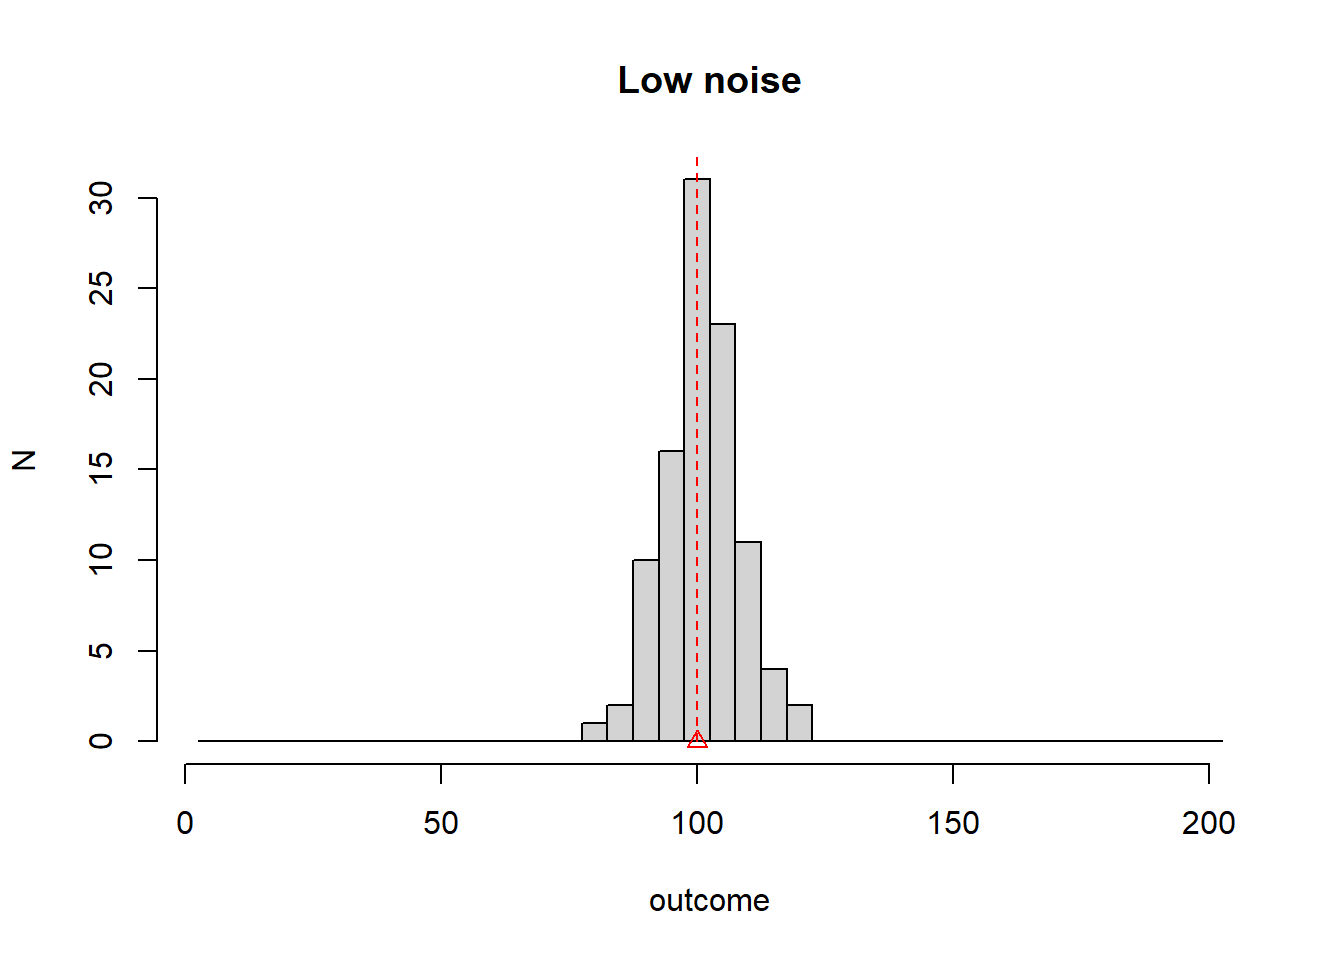
\includegraphics{_main_files/figure-latex/unnamed-chunk-22-1.pdf}

\hypertarget{probabilidad}{%
\chapter{Probabilidad}\label{probabilidad}}

\hypertarget{objetivo-2}{%
\section{Objetivo}\label{objetivo-2}}

\begin{itemize}
\tightlist
\item
  Definición de probabilidad
\item
  Álgebra de probabilidad
\item
  Probabilidad conjunta
\end{itemize}

\begin{center}\rule{0.5\linewidth}{0.5pt}\end{center}

\begin{center}\rule{0.5\linewidth}{0.5pt}\end{center}

\hypertarget{experimentos-aleatorios-1}{%
\section{Experimentos aleatorios}\label{experimentos-aleatorios-1}}

\textbf{Observación}

\begin{itemize}
\tightlist
\item
  y \textbf{observación} es la adquisición de un número o una característica de un experimento
\end{itemize}

\textbf{Salir}

\begin{itemize}
\tightlist
\item
  Un \textbf{resultado} es una posible observación que es el resultado de un experimento.
\end{itemize}

\textbf{Experimento aleatorio}

\begin{itemize}
\tightlist
\item
  Un experimento que da resultados \textbf{diferentes} cuando se repite de la misma manera.
\end{itemize}

\begin{center}\rule{0.5\linewidth}{0.5pt}\end{center}

\begin{center}\rule{0.5\linewidth}{0.5pt}\end{center}

\hypertarget{probabilidad-1}{%
\section{Probabilidad}\label{probabilidad-1}}

La \textbf{probabilidad} de un resultado es una medida de cuán seguros estamos de observar ese resultado al realizar un experimento aleatorio.

\begin{itemize}
\item
  0: Estamos seguros de que la observación \textbf{no} ocurrirá.
\item
  1: Estamos seguros de que la observación sucederá.
\end{itemize}

\begin{center}\rule{0.5\linewidth}{0.5pt}\end{center}

\begin{center}\rule{0.5\linewidth}{0.5pt}\end{center}

\hypertarget{ejemplo-3}{%
\section{Ejemplo}\label{ejemplo-3}}

\begin{itemize}
\tightlist
\item
  Considere las siguientes observaciones de un experimento aleatorio:
\end{itemize}

1 5 1 2 2 1 2 2

\begin{itemize}
\tightlist
\item
  ¿Qué tan seguro estamos de obtener \(2\) en la siguiente observación?
\end{itemize}

\begin{center}\rule{0.5\linewidth}{0.5pt}\end{center}

\begin{center}\rule{0.5\linewidth}{0.5pt}\end{center}

\hypertarget{ejemplo-4}{%
\section{Ejemplo}\label{ejemplo-4}}

La tabla de frecuencias es

\begin{verbatim}
##   outcome ni    fi
## 1       1  3 0.375
## 2       2  4 0.500
## 3       5  1 0.125
\end{verbatim}

La \textbf{frecuencia relativa} \(f_i\)

\begin{itemize}
\tightlist
\item
  es un número entre \(0\) y \(1\).
\item
  mide la proporción del total de observaciones que observamos un resultado particular.
\item
  parece una medida de probabilidad razonable.
\end{itemize}

Como \(f_2=0.5\) entonces estaríamos \(50º%
\) seguros de obtener \(2\) en la siguiente repetición del experimento.

\begin{center}\rule{0.5\linewidth}{0.5pt}\end{center}

\begin{center}\rule{0.5\linewidth}{0.5pt}\end{center}

\hypertarget{frecuencia-relativa}{%
\section{Frecuencia relativa}\label{frecuencia-relativa}}

¿\(f_i\) es una buena medida de certeza?

Digamos que repetimos el experimento 12 veces más:

1 5 1 2 2 1 2 2 \textbf{3 1 1 3 3 1 6 3 5 6 4 4}

La tabla de frecuencias es ahora

\begin{verbatim}
##   outcome ni  fi
## 1       1  6 0.3
## 2       2  4 0.2
## 3       3  4 0.2
## 4       4  2 0.1
## 5       5  2 0.1
## 6       6  2 0.1
\end{verbatim}

Aparecieron nuevos resultados y \(f_2\) ahora es \(0.2\), ahora estamos un \(20\%\) seguros de obtener \(2\) en el próximo experimento\ldots{} la probabilidad no debería depender de \(N\)

\begin{center}\rule{0.5\linewidth}{0.5pt}\end{center}

\begin{center}\rule{0.5\linewidth}{0.5pt}\end{center}

\hypertarget{en-el-infinito}{%
\section{En el infinito}\label{en-el-infinito}}

Digamos que repetimos el experimento 1000 veces:

\begin{verbatim}
##   outcome  ni    fi
## 1       1 160 0.160
## 2       2 142 0.142
## 3       3 163 0.163
## 4       4 169 0.169
## 5       5 163 0.163
## 6       6 203 0.203
\end{verbatim}

Encontramos que \(f_i\) está convergiendo a un valor constante

\[lim_{N\rightarrow \infty} f_i = P_i\]

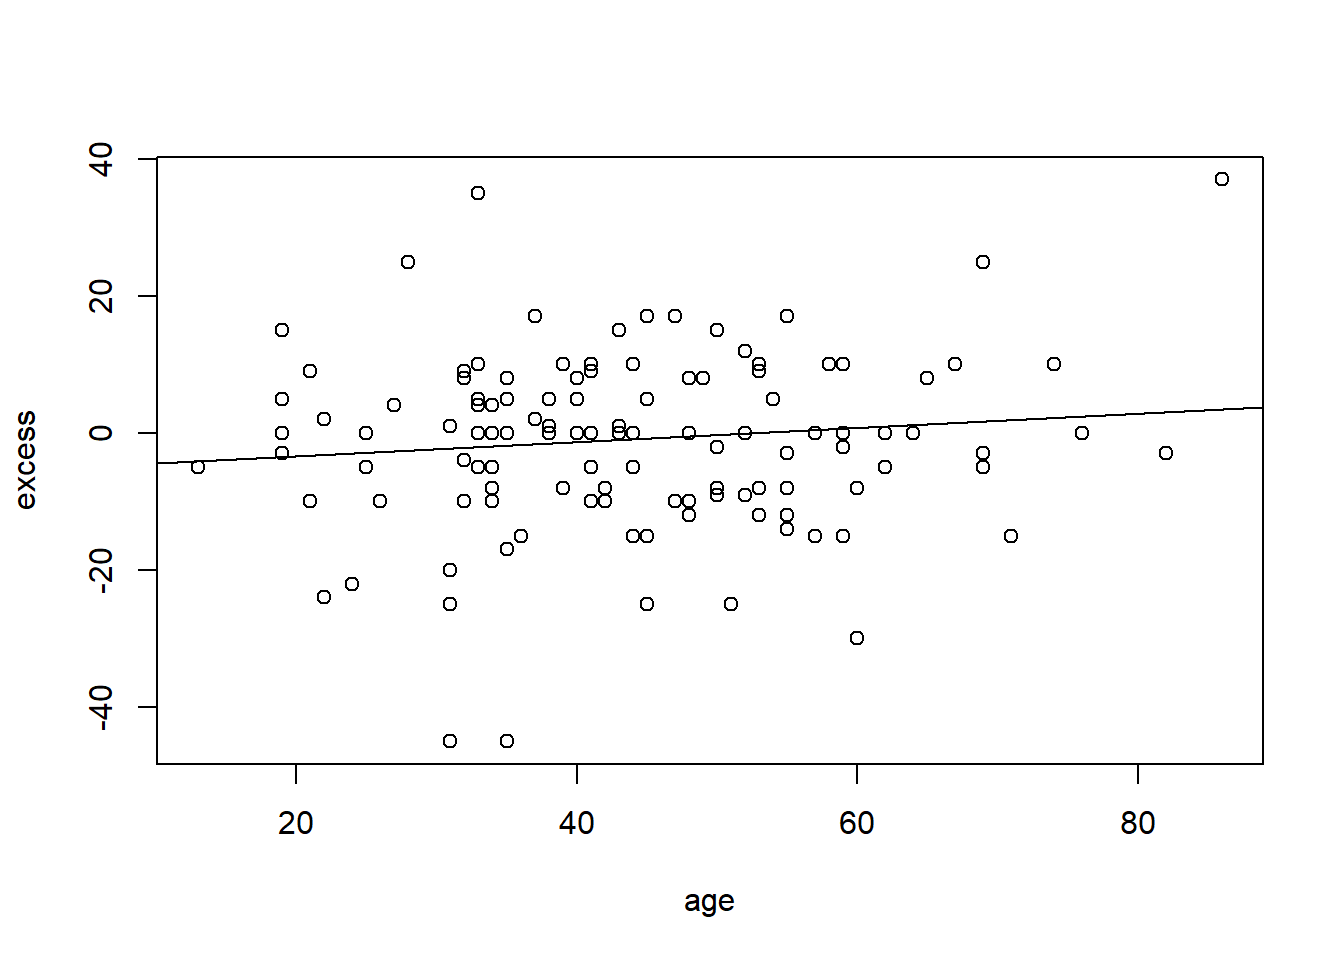
\includegraphics{_main_files/figure-latex/unnamed-chunk-26-1.pdf}

\begin{center}\rule{0.5\linewidth}{0.5pt}\end{center}

\begin{center}\rule{0.5\linewidth}{0.5pt}\end{center}

\hypertarget{probabilidad-frecuentista}{%
\section{Probabilidad frecuentista}\label{probabilidad-frecuentista}}

Llamamos \textbf{Probabilidad} \(P_i\) al límite cuando \(N \rightarrow \infty\) de la \textbf{frecuencia relativa} de observar el resultado \(i\) en un experimento aleatorio.

Defendida por \href{https://plato.stanford.edu/entries/probability-interpret/\#ClaPro}{Venn (1876)}

La interpretación frecuentista de probabilidades se deriva de datos/experiencia (empírica).

\begin{itemize}
\tightlist
\item
  No observamos \(P_i\), observamos \(f_i\)
\item
  Cuando \textbf{estimamos} \(P_i\) con \(f_i\) (normalmente cuando \(N\) es grande), escribimos: \[\hat{P_i}=f_i\]
\end{itemize}

\begin{center}\rule{0.5\linewidth}{0.5pt}\end{center}

\begin{center}\rule{0.5\linewidth}{0.5pt}\end{center}

\hypertarget{probabilidad-cluxe1sica}{%
\section{Probabilidad clásica}\label{probabilidad-cluxe1sica}}

Cada vez que un experimento aleatorio tiene \(M\) resultados posibles que son todos \textbf{igualmente probables}, la probabilidad de cada resultado es \(\frac{1}{M}\).

Defendida por \href{https://plato.stanford.edu/entries/probability-interpret/\#ClaPro}{Laplace (1814)}.

Dado que cada resultado es \textbf{igualmente probable}, declaramos una completa ignorancia y lo mejor que podemos hacer es distribuir equitativamente la misma probabilidad para cada resultado.

¿Y si te dijera que nuestro experimento fue tirar un dado? entonces

\(P_2=1/6=0.166666\).

\[P_i=lim_{N\rightarrow \infty} \frac{n_i}{N}=\frac{1}{M}\]

\begin{center}\rule{0.5\linewidth}{0.5pt}\end{center}

\begin{center}\rule{0.5\linewidth}{0.5pt}\end{center}

\hypertarget{probabilidades-cluxe1sicas-y-frecuentistas}{%
\section{Probabilidades clásicas y frecuentistas}\label{probabilidades-cluxe1sicas-y-frecuentistas}}

\begin{center}\rule{0.5\linewidth}{0.5pt}\end{center}

\begin{center}\rule{0.5\linewidth}{0.5pt}\end{center}

\hypertarget{probabilidad-2}{%
\section{Probabilidad}\label{probabilidad-2}}

La probabilidad es un número entre \(0\) y \(1\) que se asigna a cada miembro \(E\) de una colección de \textbf{eventos} de un \textbf{espacio muestral} (\(S\)) de un experimento aleatorio.

\[P(E) \in (0,1)\]

donde \(E \in S\)

\begin{center}\rule{0.5\linewidth}{0.5pt}\end{center}

\begin{center}\rule{0.5\linewidth}{0.5pt}\end{center}

\hypertarget{espacio-muestral}{%
\section{Espacio muestral}\label{espacio-muestral}}

Empezamos razonando cuáles son todos los valores posibles (resultados) que podría dar un experimento aleatorio.

Tenga en cuenta que no tenemos que observarlos en un experimento en particular: estamos usando \textbf{razón/lógica} y no observación.

\textbf{Definición:}

\begin{itemize}
\item
  El conjunto de todos los resultados posibles de un experimento aleatorio se denomina \textbf{espacio muestral}
  del experimento
\item
  El espacio muestral se denota como \(S\).
\end{itemize}

\begin{center}\rule{0.5\linewidth}{0.5pt}\end{center}

\begin{center}\rule{0.5\linewidth}{0.5pt}\end{center}

\hypertarget{ejemplos-de-espacios-muestrales}{%
\section{Ejemplos de espacios muestrales}\label{ejemplos-de-espacios-muestrales}}

\begin{itemize}
\tightlist
\item
  temperatura 35 y 42 grados centígrados
\item
  niveles de azúcar: 70-80mg/dL
\item
  el tamaño de un tornillo de una línea de producción: 70 mm-72 mm
\item
  número de correos electrónicos recibidos en una hora: 0-100
\item
  un lanzamiento de dados: 1, 2, 3, 4, 5, 6
\end{itemize}

\begin{center}\rule{0.5\linewidth}{0.5pt}\end{center}

\begin{center}\rule{0.5\linewidth}{0.5pt}\end{center}

\hypertarget{espacios-muestrales-discretos-y-continuos}{%
\section{Espacios muestrales discretos y continuos}\label{espacios-muestrales-discretos-y-continuos}}

\begin{itemize}
\item
  Un espacio muestral es discreto si consiste en un conjunto de resultados finito o infinito numerable.
\item
  Un espacio muestral es continuo si contiene un intervalo (ya sea de longitud finita o infinita) de
  numeros reales.
\end{itemize}

\begin{center}\rule{0.5\linewidth}{0.5pt}\end{center}

\begin{center}\rule{0.5\linewidth}{0.5pt}\end{center}

\hypertarget{evento}{%
\section{Evento}\label{evento}}

\textbf{Definición:}

Un \textbf{evento} es un \textbf{subconjunto} del espacio muestral de un experimento aleatorio. Es una \textbf{colección} de resultados.

Ejemplos de eventos:

\begin{itemize}
\tightlist
\item
  El evento de una temperatura saludable: temperatura 37-38 grados centígrados
\item
  El evento de producir un tornillo con un tamaño: de 71,5 mm
\item
  El evento de recibir más de 4 correos electrónicos en una hora.
\item
  El evento de obtener un número menor de 3 en el lanzamiento de un dado
\end{itemize}

Un evento se refiere a un posible conjunto de \textbf{resultados}.

\begin{center}\rule{0.5\linewidth}{0.5pt}\end{center}

\begin{center}\rule{0.5\linewidth}{0.5pt}\end{center}

\hypertarget{operaciones-de-eventos}{%
\section{Operaciones de eventos}\label{operaciones-de-eventos}}

Para dos eventos \(A\) y \(B\), podemos construir los siguientes eventos derivados:

\begin{itemize}
\tightlist
\item
  Complemento \(A'\): el evento de \textbf{no} \(A\)
\item
  Unión \(A \cup B\): el evento de \(A\) \textbf{o} \(B\)
\item
  Intersección \(A \cap B\): el evento de \(A\) \textbf{y} \(B\)
\end{itemize}

\begin{center}\rule{0.5\linewidth}{0.5pt}\end{center}

\begin{center}\rule{0.5\linewidth}{0.5pt}\end{center}

\hypertarget{ejemplo-de-operaciones-de-eventos}{%
\section{Ejemplo de operaciones de eventos}\label{ejemplo-de-operaciones-de-eventos}}

Tomar

\begin{itemize}
\tightlist
\item
  Evento \(A:\{1,2,3\}\) un número menor o igual a tres en el lanzamiento de un dado
\item
  Evento \(B:\{2,4,6\}\) un número par en el lanzamiento de un dado
\end{itemize}

Nuevos eventos:

\begin{itemize}
\tightlist
\item
  No menos de tres: \(A':\{4,5,6\}\)
\item
  Menor o igual a tres \textbf{o} par: \(A \cup B: \{1,2,3,4,6\}\)
\item
  Menor o igual a tres \textbf{y} par \(A \cap B: \{2\}\)
\end{itemize}

\begin{center}\rule{0.5\linewidth}{0.5pt}\end{center}

\begin{center}\rule{0.5\linewidth}{0.5pt}\end{center}

\hypertarget{resultados}{%
\section{Resultados}\label{resultados}}

Los resultados son eventos que son \textbf{mutuamente excluyentes}

\textbf{Definición:}

Dos eventos denotados como \(E_1\) y \(E_2\), tales que

\[E_1\cap E_2=\emptyset\]
No pueden ocurrir al mismo tiempo.

Ejemplo:

\begin{itemize}
\item
  El resultado de obtener \(1\) \textbf{y} el resultado de obtener \(5\) en el lanzamiento de un dado son mutuamente excluyentes:
\item
  El evento de obtener \(1\) y \(5\) está vacío:\[\{1\}\cap \{5\}=\emptyset\]
\end{itemize}

\begin{center}\rule{0.5\linewidth}{0.5pt}\end{center}

\begin{center}\rule{0.5\linewidth}{0.5pt}\end{center}

\hypertarget{definiciuxf3n-de-probabilidad}{%
\section{Definición de probabilidad}\label{definiciuxf3n-de-probabilidad}}

Una probabilidad es un número que se asigna a cada evento posible (\(E\)) de un espacio muestral (\(S\)) de un experimento aleatorio que cumple las siguientes propiedades:

\begin{itemize}
\tightlist
\item
  \(P(S)=1\)
\item
  \(0 \leq P(E) \leq 1\)
\item
  cuando \(E_1\cap E_2=\emptyset\) \[P(E_1\cup E_2) = P(E_1) + P(E_2)\]
\end{itemize}

Propuesto por Kolmogorov (1933)

\begin{center}\rule{0.5\linewidth}{0.5pt}\end{center}

\begin{center}\rule{0.5\linewidth}{0.5pt}\end{center}

\hypertarget{propiedades-de-probabilidad}{%
\section{Propiedades de probabilidad}\label{propiedades-de-probabilidad}}

Kolmogorov dice que podemos construir una tabla de probabilidad (al igual que la tabla de frecuencia relativa)

\begin{longtable}[]{@{}cc@{}}
\toprule
resultado & Probabilidad \\
\midrule
\endhead
\(1\) & 1/6 \\
\(2\) & 1/6 \\
\(3\) & 1/6 \\
\(4\) & 1/6 \\
\(5\) & 1/6 \\
\(6\) & 1/6 \\
\(P(1\cup 2\cup ...\cup 6)\) & 1 \\
\bottomrule
\end{longtable}

Como \(\{1,2,3,4,5,6\}\) son mutuamente excluyentes, entonces

\[P(S)=P(1\cup 2\cup ...\cup 6) = P(1)+P(2)+ ...+P(n)=1\]

\begin{center}\rule{0.5\linewidth}{0.5pt}\end{center}

\begin{center}\rule{0.5\linewidth}{0.5pt}\end{center}

\hypertarget{regla-de-adiciuxf3n}{%
\section{Regla de adición}\label{regla-de-adiciuxf3n}}

Cuando \(A\) y \(B\) no son mutuamente excluyentes, entonces:

\[P(A\cup B)=P(A) + P(B) - P(A\cap B)\]

Donde \(P(A)\) y \(P(B)\) se denominan \textbf{probabilidades marginales}

\begin{center}\rule{0.5\linewidth}{0.5pt}\end{center}

\begin{center}\rule{0.5\linewidth}{0.5pt}\end{center}

\hypertarget{ejemplo-de-regla-de-adiciuxf3n}{%
\section{Ejemplo de regla de adición}\label{ejemplo-de-regla-de-adiciuxf3n}}

Tomar

\begin{itemize}
\tightlist
\item
  Evento \(A:\{1,2,3\}\) un número menor o igual a tres en el lanzamiento de un dado
\item
  Evento \(B:\{2,4,6\}\) un número par en el lanzamiento de un dado
\end{itemize}

después:

\begin{itemize}
\tightlist
\item
  \(P(A): P(1) + P(2) + P(3)=3/6\)
\item
  \(P(G): P(2) + P(4) + P(6)=3/6\)
\item
  \(P(A \cap B): P(2) = 1/6\)
\end{itemize}

\(P(A\cup B)=P(A) + P(B) - P(A\cap B)=3/6+3/6-1/6=5/6\)

Nota: \(P(2)\) aparece en \(P(A)\) y \(P(B)\) por eso lo restamos con la intersección

\begin{center}\rule{0.5\linewidth}{0.5pt}\end{center}

\begin{center}\rule{0.5\linewidth}{0.5pt}\end{center}

\hypertarget{diagrama-de-venn}{%
\section{Diagrama de Venn}\label{diagrama-de-venn}}

Tenga en cuenta que siempre se puede descomponer el espacio muestral en conjuntos \textbf{mutuamente excluyentes} que involucran las intersecciones:

\(S=\{A\cap B, A \cap B', A'\cap B, A'\cap B'\}\)

Marginales:

\begin{itemize}
\tightlist
\item
  \(P(A)=P(A\cap B') + P(A \cap B)=2/6+1/6=3/6\)
\item
  \(P(B)=P(A'\cap B) +P(A \cap B)=2/6+1/6=3/6\)
\end{itemize}

\begin{center}\rule{0.5\linewidth}{0.5pt}\end{center}

\begin{center}\rule{0.5\linewidth}{0.5pt}\end{center}

\hypertarget{tabla-de-probabilidades}{%
\section{Tabla de probabilidades}\label{tabla-de-probabilidades}}

Veamos la tabla de probabilidades.

\begin{longtable}[]{@{}cc@{}}
\toprule
resultado & Probabilidad \\
\midrule
\endhead
\(A\cap B\) & \(P(A\cap B)\) \\
\(A\cap B'\) & \(P(A\cap B')\) \\
\(A'\cap B\) & \(P(A'\cap B)\) \\
\(A'\cap B'\) & \(P(A'\cap B')\) \\
suma & \(1\) \\
\bottomrule
\end{longtable}

\begin{center}\rule{0.5\linewidth}{0.5pt}\end{center}

\begin{center}\rule{0.5\linewidth}{0.5pt}\end{center}

\hypertarget{ejemplo-de-tabla-de-probabilidades}{%
\section{Ejemplo de tabla de probabilidades}\label{ejemplo-de-tabla-de-probabilidades}}

También escribimos \(A \cap B\) como \((A,B)\) y lo llamamos la \textbf{probabilidad conjunta} de \(A\) y \(B\)

En nuestro ejemplo:

\begin{longtable}[]{@{}cc@{}}
\toprule
resultado & Probabilidad \\
\midrule
\endhead
\((A,B)\) & \(P(A, B)=1/6\) \\
\((A,B')\) & \(P(A,B')=2/6\) \\
\((A', B)\) & \(P(A', B)=2/6\) \\
\((A', B')\) & \(P(A', B')=1/6\) \\
suma & \(1\) \\
\bottomrule
\end{longtable}

Nota: cada resultado tiene \(dos\) valores (uno para la característica del tipo \(A\) y otro para el tipo \(B\))

\begin{center}\rule{0.5\linewidth}{0.5pt}\end{center}

\begin{center}\rule{0.5\linewidth}{0.5pt}\end{center}

\hypertarget{mesa-de-contingencia}{%
\section{Mesa de contingencia}\label{mesa-de-contingencia}}

Podemos organizar la probabilidad de \textbf{resultados conjuntos} en una \textbf{tabla de contingencia}

\begin{longtable}[]{@{}cccc@{}}
\toprule
& \(B\) & \(B'\) & suma \\
\midrule
\endhead
\(A\) & \(P(A, B )\) & \(P(A, B' )\) & \(P(A)\) \\
\(A'\) & \(P(A', B )\) & \(P(A', B' )\) & \(P(A')\) \\
suma & \(P(B)\) & \(P(B')\) & 1 \\
\bottomrule
\end{longtable}

marginales:

\begin{itemize}
\tightlist
\item
  \(P(A)=P(A, B') + P(A, B)\)
\item
  \(P(B)=P(A', B) +P(A, B)\)
\end{itemize}

\begin{center}\rule{0.5\linewidth}{0.5pt}\end{center}

\begin{center}\rule{0.5\linewidth}{0.5pt}\end{center}

\hypertarget{ejemplo-de-tabla-de-contingencia}{%
\section{Ejemplo de tabla de contingencia}\label{ejemplo-de-tabla-de-contingencia}}

\begin{itemize}
\tightlist
\item
  Evento \(A:\{1,2,3\}\) un número menor o igual a tres en el lanzamiento de un dado
\item
  Evento \(B:\{2,4,6\}\) un número par en el lanzamiento de un dado
\end{itemize}

\begin{longtable}[]{@{}cccc@{}}
\toprule
& \(B\) & \(B'\) & suma \\
\midrule
\endhead
\(A\) & \(1/6\) & \(2/6\) & \(3/6\) \\
\(A'\) & \(2/6\) & \(1/6\) & \(3/6\) \\
suma & \(3/6\) & \(3/6\) & 1 \\
\bottomrule
\end{longtable}

Tres formas de la \textbf{regla de la suma}:

\(P(A\cup B)\)\[=P(A) + P(B) - P(A\cap B)\]
\[=P(A \cap B)+P(A\cap B')+P(A\cap B')\]
\[=1-P(A'\cap B')\]

\begin{center}\rule{0.5\linewidth}{0.5pt}\end{center}

\begin{center}\rule{0.5\linewidth}{0.5pt}\end{center}

\hypertarget{estudio-de-misofonuxeda}{%
\section{Estudio de misofonía}\label{estudio-de-misofonuxeda}}

En el estudio de misofonía, se evaluó a los pacientes según la gravedad de su misofonía \textbf{y} si estaban deprimidos.

El resultado de un experimento aleatorio es medir la gravedad de la misofonía \textbf{y} el estado de depresión de un paciente. La repetición del experimento aleatorio consistía en realizar las mismas dos mediciones en otro paciente.

\begin{verbatim}
##     Misofonia.dic depresion.dic
## 1               4             1
## 2               2             0
## 3               0             0
## 4               3             0
## 5               0             0
## 6               0             0
## 7               2             0
## 8               3             0
## 9               0             1
## 10              3             0
## 11              0             0
## 12              2             0
## 13              2             1
## 14              0             0
## 15              2             0
## 16              0             0
## 17              0             0
## 18              3             0
## 19              3             0
## 20              0             0
## 21              3             0
## 22              3             0
## 23              2             0
## 24              0             0
## 25              0             0
## 26              0             0
## 27              4             1
## 28              2             0
## 29              2             0
## 30              0             0
## 31              2             0
## 32              0             0
## 33              0             0
## 34              0             0
## 35              3             0
## 36              0             0
## 37              2             0
## 38              3             1
## 39              2             0
## 40              2             0
## 41              0             0
## 42              2             0
## 43              3             0
## 44              0             0
## 45              0             0
## 46              2             0
## 47              2             0
## 48              3             0
## 49              3             0
## 50              0             0
## 51              0             0
## 52              4             1
## 53              3             0
## 54              3             1
## 55              2             1
## 56              0             1
## 57              2             0
## 58              0             0
## 59              0             0
## 60              0             0
## 61              2             0
## 62              2             0
## 63              0             0
## 64              0             0
## 65              2             0
## 66              3             1
## 67              0             0
## 68              1             0
## 69              3             0
## 70              2             0
## 71              4             1
## 72              3             0
## 73              2             1
## 74              3             0
## 75              0             1
## 76              2             0
## 77              3             0
## 78              2             0
## 79              4             1
## 80              1             0
## 81              2             0
## 82              0             0
## 83              2             0
## 84              0             0
## 85              2             0
## 86              0             1
## 87              2             0
## 88              2             0
## 89              4             1
## 90              3             0
## 91              0             1
## 92              3             0
## 93              0             0
## 94              0             0
## 95              0             0
## 96              2             0
## 97              2             0
## 98              1             0
## 99              3             0
## 100             0             0
## 101             0             0
## 102             3             1
## 103             2             0
## 104             1             0
## 105             3             0
## 106             0             0
## 107             4             1
## 108             4             1
## 109             2             0
## 110             3             0
## 111             3             0
## 112             3             1
## 113             0             0
## 114             3             0
## 115             2             0
## 116             1             0
## 117             2             0
## 118             3             1
## 119             3             0
## 120             4             1
## 121             2             0
## 122             3             0
## 123             2             0
\end{verbatim}

\begin{center}\rule{0.5\linewidth}{0.5pt}\end{center}

\begin{center}\rule{0.5\linewidth}{0.5pt}\end{center}

\hypertarget{tabla-de-contingencia-para-frecuencias}{%
\section{Tabla de contingencia para frecuencias}\label{tabla-de-contingencia-para-frecuencias}}

\begin{itemize}
\tightlist
\item
  Por el número de observaciones \(n_{i,j}\) de cada resultado \((x_i, y_i)\), misofonía: \(x\in \{0,1,2,3,4\}\) y depresión \(y\ en \{0,1\}\) (no:\(0\), sí:\(1\))
\end{itemize}

\begin{verbatim}
##               
##                Depression:0 Depression:1
##   Misophonia:4            0            9
##   Misophonia:3           25            6
##   Misophonia:2           34            3
##   Misophonia:1            5            0
##   Misophonia:0           36            5
\end{verbatim}

\begin{itemize}
\tightlist
\item
  For the relative frequencies \(f_{i,j}\)
\end{itemize}

\begin{verbatim}
##               
##                Depression:0 Depression:1
##   Misophonia:4   0.00000000   0.07317073
##   Misophonia:3   0.20325203   0.04878049
##   Misophonia:2   0.27642276   0.02439024
##   Misophonia:1   0.04065041   0.00000000
##   Misophonia:0   0.29268293   0.04065041
\end{verbatim}

\begin{center}\rule{0.5\linewidth}{0.5pt}\end{center}

\begin{center}\rule{0.5\linewidth}{0.5pt}\end{center}

\hypertarget{mapa-de-calor}{%
\section{Mapa de calor}\label{mapa-de-calor}}

La tabla de contingencia se puede trazar como un \textbf{mapa de calor}

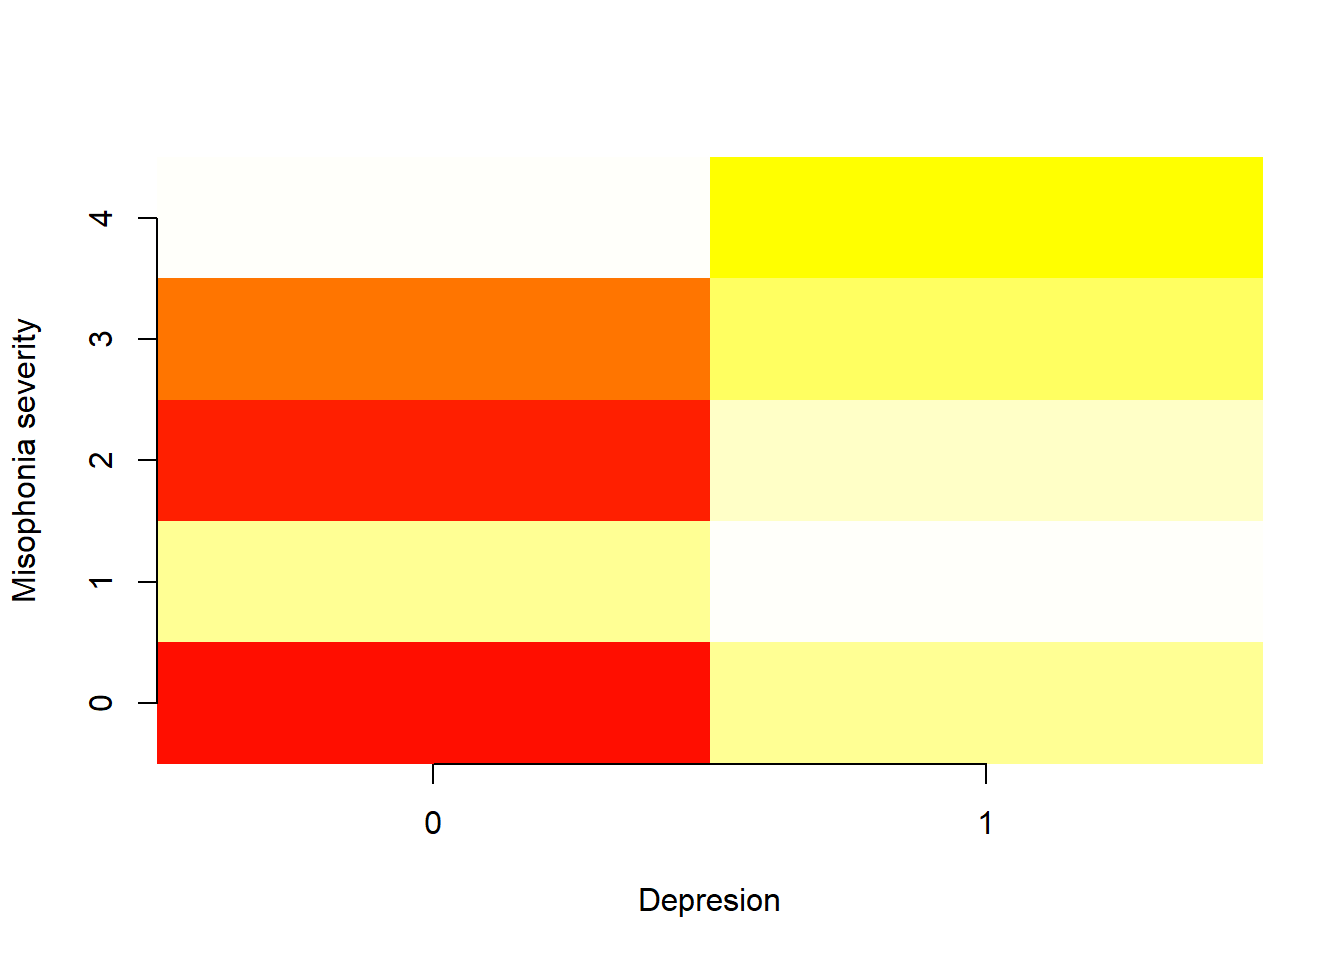
\includegraphics{_main_files/figure-latex/unnamed-chunk-30-1.pdf}

\begin{center}\rule{0.5\linewidth}{0.5pt}\end{center}

\begin{center}\rule{0.5\linewidth}{0.5pt}\end{center}

\hypertarget{variables-continuas-1}{%
\section{Variables continuas}\label{variables-continuas-1}}

En el estudio de misofonía también se midió la protrusión mandibular como posible factor cefalométrico de la enfermedad.

\begin{verbatim}
##     Angulo_convexidad protusion.mandibular
## 1                7.97                13.00
## 2               18.23                -5.00
## 3               12.27                11.50
## 4                7.81                16.80
## 5                9.81                33.00
## 6               13.50                 2.00
## 7               19.30                -3.90
## 8                7.70                16.80
## 9               12.30                 8.00
## 10               7.90                28.80
## 11              12.60                 3.00
## 12              19.00                -7.90
## 13               7.27                28.30
## 14              14.00                 4.00
## 15               5.40                22.20
## 16               8.00                 0.00
## 17              11.20                15.00
## 18               7.75                17.00
## 19               7.94                49.00
## 20              16.69                 5.00
## 21               7.62                42.00
## 22               7.02                28.00
## 23               7.00                 9.40
## 24              19.20               -13.20
## 25               7.96                23.00
## 26              14.70                 2.30
## 27               7.24                25.00
## 28               7.80                 4.90
## 29               7.90                92.00
## 30               4.70                 6.00
## 31               4.40                17.00
## 32              14.00                 3.30
## 33              14.40                10.30
## 34              16.00                 6.30
## 35               1.40                19.50
## 36               9.76                22.00
## 37               7.90                 5.00
## 38               7.90                78.00
## 39               7.40                 9.30
## 40               6.30                50.60
## 41               7.76                18.00
## 42               7.30                18.00
## 43               7.00                10.00
## 44              11.23                 4.00
## 45              16.00                13.30
## 46               7.90                48.00
## 47               7.29                23.50
## 48               6.91                37.60
## 49               7.10                15.00
## 50              13.40                 5.10
## 51              11.60                -2.20
## 52              -1.00                32.00
## 53               6.00                25.00
## 54               7.82                24.00
## 55               4.80                33.60
## 56              11.00                 3.30
## 57               9.00                31.50
## 58              11.50                12.80
## 59              16.00                 3.00
## 60              15.00                 6.00
## 61               1.40                21.40
## 62              16.80               -10.00
## 63               7.70                19.00
## 64              16.14                32.00
## 65               7.12                15.00
## 66              -1.00                10.00
## 67              17.00               -16.90
## 68               9.26                 2.00
## 69              18.70               -10.10
## 70               3.40                12.20
## 71              21.30               -11.00
## 72               7.50                 5.20
## 73               6.03                16.00
## 74               7.50                 5.80
## 75              19.00                 5.20
## 76              19.01                13.00
## 77               8.10                13.60
## 78               7.80                16.10
## 79               6.10                33.20
## 80              15.26                 4.00
## 81               7.95                12.00
## 82              18.00                -1.50
## 83               4.60                18.30
## 84              15.00                 3.00
## 85               7.50                15.80
## 86               8.00                27.10
## 87              16.80               -10.00
## 88               8.54                25.00
## 89               7.00                27.10
## 90              18.30                -8.00
## 91               7.80                12.00
## 92              16.00                -8.00
## 93              14.00                23.00
## 94              12.30                 5.00
## 95              11.40                 1.00
## 96               8.50                18.90
## 97               7.00                15.00
## 98               7.96                22.00
## 99              17.60                -3.50
## 100             10.00                20.00
## 101              3.50                12.20
## 102              6.70                14.70
## 103             17.00                -5.00
## 104             20.26                -4.15
## 105              6.64                11.00
## 106              1.80                -4.00
## 107              7.02                25.00
## 108              2.46                35.00
## 109             19.00                -5.00
## 110             17.86               -30.00
## 111              6.10                12.20
## 112              6.64                19.00
## 113             12.00                 1.60
## 114              6.60                20.00
## 115              8.70                17.10
## 116             14.05                24.00
## 117              7.20                 7.10
## 118             19.70               -11.00
## 119              7.70                21.30
## 120              6.02                 5.00
## 121              2.50                12.90
## 122             19.00                 5.90
## 123              6.80                 5.80
\end{verbatim}

\begin{center}\rule{0.5\linewidth}{0.5pt}\end{center}

\begin{center}\rule{0.5\linewidth}{0.5pt}\end{center}

\hypertarget{variables-continuas-2}{%
\section{Variables continuas}\label{variables-continuas-2}}

En el estudio de misofonía también se midió la protrusión mandibular como posible factor cefalométrico de la enfermedad.

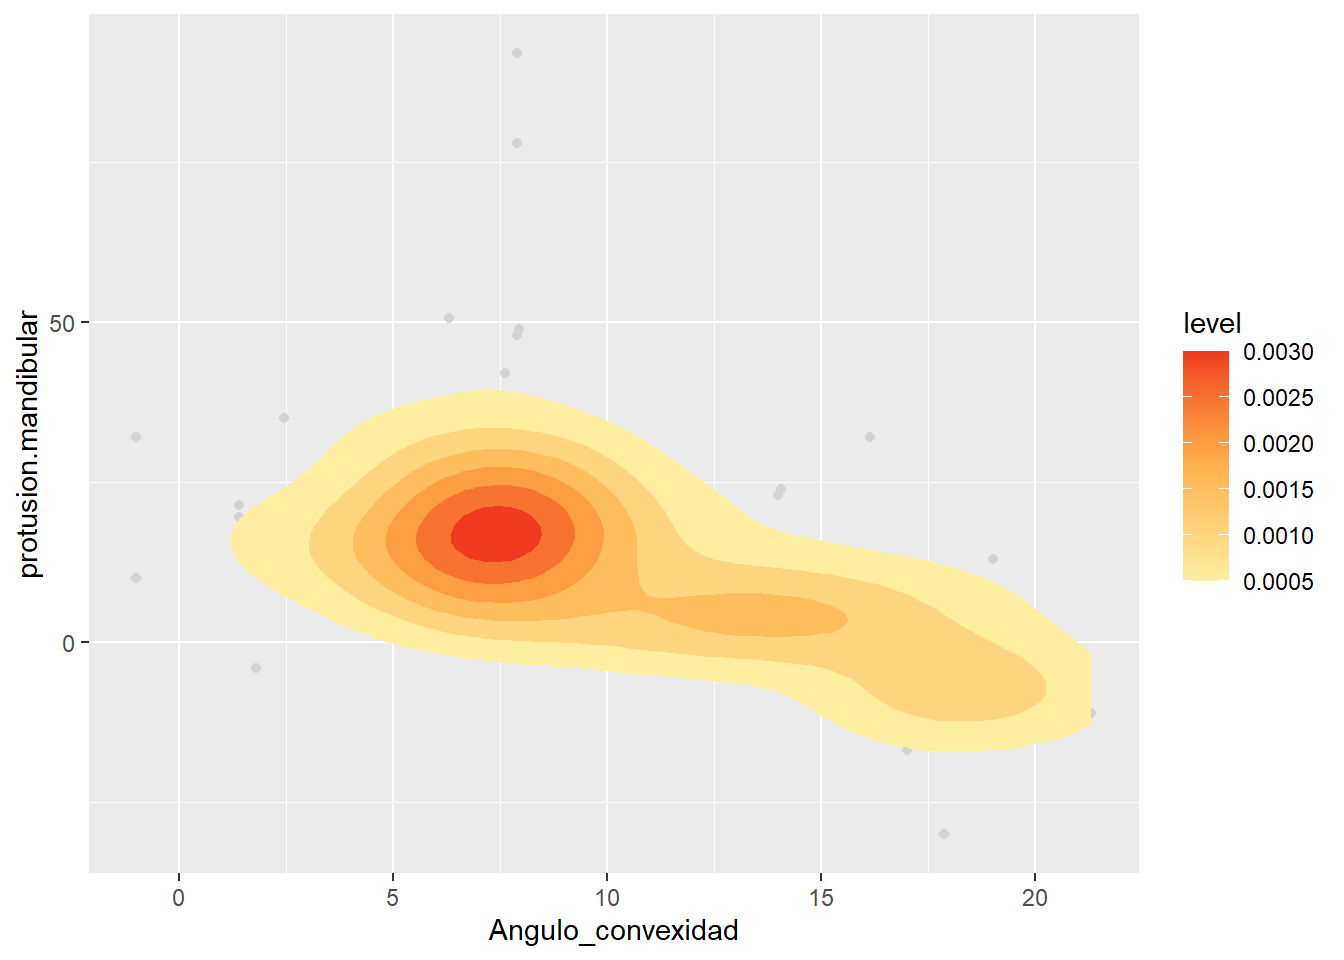
\includegraphics{_main_files/figure-latex/unnamed-chunk-32-1.pdf}

\begin{center}\rule{0.5\linewidth}{0.5pt}\end{center}

\begin{center}\rule{0.5\linewidth}{0.5pt}\end{center}

\hypertarget{gruxe1fico-de-dispersiuxf3n}{%
\section{Gráfico de dispersión}\label{gruxe1fico-de-dispersiuxf3n}}

\begin{itemize}
\item
  El \textbf{histograma} depende del tamaño del contenedor (píxel).
\item
  Si el píxel es lo suficientemente pequeño como para contener una sola observación, el mapa de calor da como resultado un \textbf{diagrama de dispersión}
\end{itemize}

El diagrama de dispersión es la ilustración de una ``tabla de contingencia'' para variables continuas cuando el contenedor (píxel) es lo suficientemente pequeño como para contener una sola observación (que consta de un par de valores).

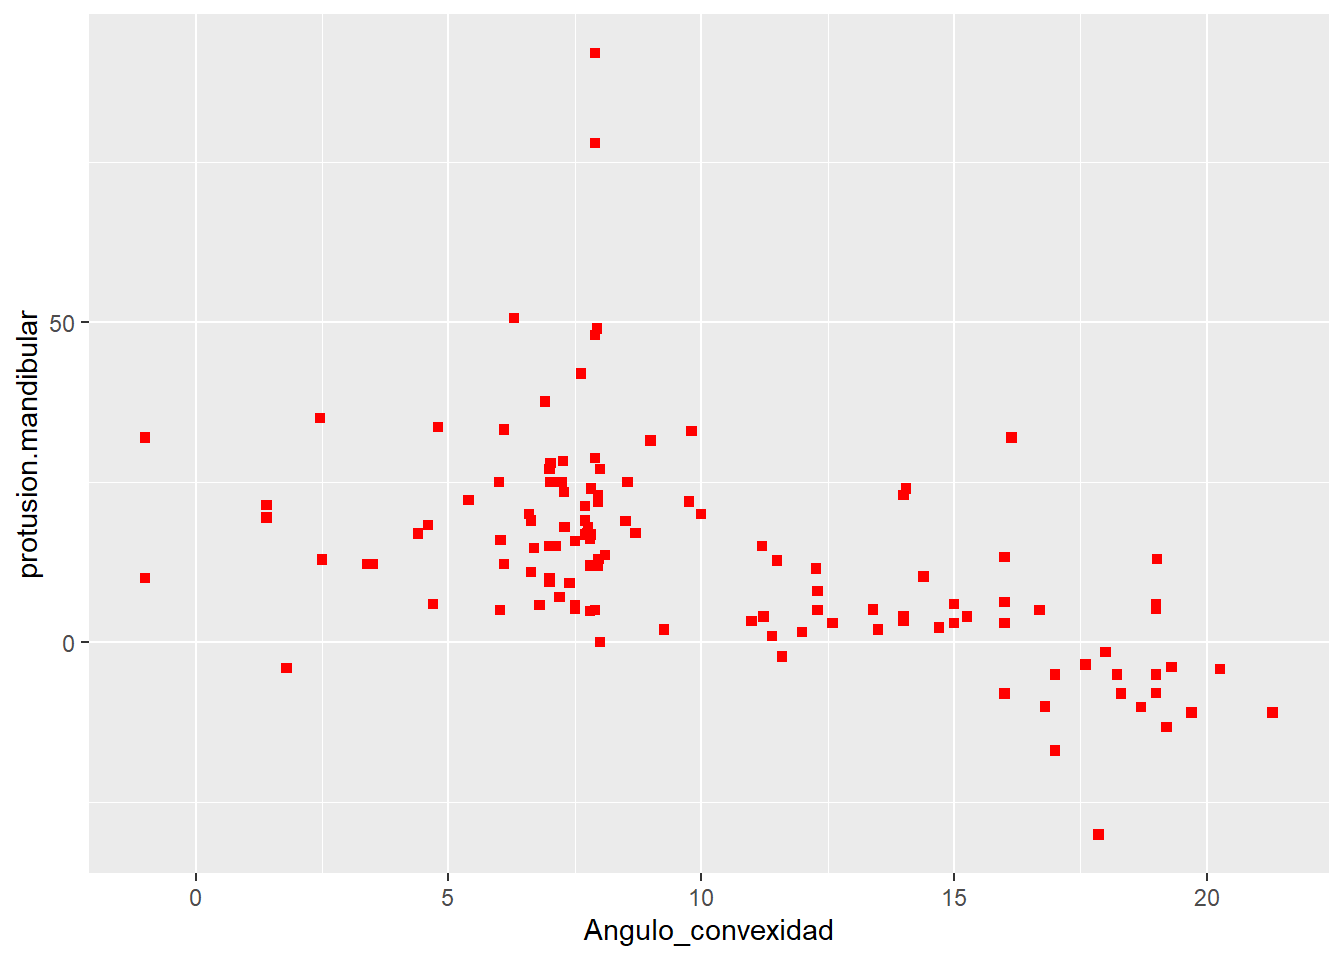
\includegraphics{_main_files/figure-latex/unnamed-chunk-33-1.pdf}

\hypertarget{probabilidad-condicional}{%
\chapter{Probabilidad condicional}\label{probabilidad-condicional}}

\hypertarget{objetivo-3}{%
\section{Objetivo}\label{objetivo-3}}

\begin{itemize}
\tightlist
\item
  Probabilidad condicional
\item
  Independencia
\item
  Teorema de Bayes
\end{itemize}

\begin{center}\rule{0.5\linewidth}{0.5pt}\end{center}

\begin{center}\rule{0.5\linewidth}{0.5pt}\end{center}

\hypertarget{probabilidad-conjunta}{%
\section{Probabilidad conjunta}\label{probabilidad-conjunta}}

La probabilidad conjunta de dos eventos \(A\) y \(B\) es
\[P(A,B)=P(A \cap B)\]

Imaginemos un experimento aleatorio que mide dos tipos diferentes de resultados.

\begin{itemize}
\item
  altura y peso de un individuo: \((h, w)\)
\item
  hora y lugar de una carga eléctrica: \((p, t)\)
\item
  una tirada de dos dados: (\(n_1\),\(n_2\))
\item
  cruzar dos semáforos en verde: (\(\bar{R_1}\), \(\bar{R_2}\))
\end{itemize}

En muchos casos, nos interesa saber si los valores de un resultado \textbf{condicionan} los valores del otro.

\begin{center}\rule{0.5\linewidth}{0.5pt}\end{center}

\begin{center}\rule{0.5\linewidth}{0.5pt}\end{center}

\hypertarget{diagnuxf3sticos}{%
\section{Diagnósticos}\label{diagnuxf3sticos}}

Consideremos una \textbf{herramienta de diagnóstico}

Queremos encontrar el estado de un sistema (s):

\begin{itemize}
\tightlist
\item
  inadecuado (sí)
\item
  adecuado (no)
\end{itemize}

con una prueba (t):

\begin{itemize}
\tightlist
\item
  positivo
\item
  negativo
\end{itemize}

Probamos una batería para saber cuánto tiempo puede vivir. Tensamos un cable para saber si resiste llevar cierta carga. Realizamos una PCR para ver si alguien está infectado.

\begin{center}\rule{0.5\linewidth}{0.5pt}\end{center}

\begin{center}\rule{0.5\linewidth}{0.5pt}\end{center}

\hypertarget{prueba-de-diagnuxf3stico}{%
\section{Prueba de diagnóstico}\label{prueba-de-diagnuxf3stico}}

Consideremos diagnosticar una infección con una nueva prueba.

Estado de infección:

\begin{itemize}
\tightlist
\item
  si (infectado)
\item
  no (no infectado)
\end{itemize}

Prueba:

\begin{itemize}
\tightlist
\item
  positivo
\item
  negativo
\end{itemize}

\begin{center}\rule{0.5\linewidth}{0.5pt}\end{center}

\begin{center}\rule{0.5\linewidth}{0.5pt}\end{center}

\hypertarget{observaciones}{%
\section{Observaciones}\label{observaciones}}

Cada individuo es un experimento aleatorio con dos medidas: (Infección, Prueba)

\begin{longtable}[]{@{}ccc@{}}
\toprule
Asunto & Infección & Prueba \\
\midrule
\endhead
\(s_1\) & si & positivo \\
\(s_2\) & no & negativo \\
\(s_3\) & si & positivo \\
\ldots{} & \ldots{} & \ldots{} \\
\(s_i\) & no & positivo* \\
\ldots{} & \ldots{} & \ldots{} \\
\ldots{} & \ldots{} & \ldots{} \\
\(s_n\) & si & negativo* \\
\bottomrule
\end{longtable}

\begin{center}\rule{0.5\linewidth}{0.5pt}\end{center}

\begin{center}\rule{0.5\linewidth}{0.5pt}\end{center}

\hypertarget{tablas-de-contingencia}{%
\section{Tablas de contingencia}\label{tablas-de-contingencia}}

\begin{itemize}
\tightlist
\item
  Por el número de observaciones de cada resultado
\end{itemize}

\begin{longtable}[]{@{}cccc@{}}
\toprule
& Infección: sí & Infección: sí & suma \\
\midrule
\endhead
Test: positivo & 18 & 12 & 30 \\
Test: negativo & 30 & 300 & 330 \\
suma & 48 & 312 & 360 \\
\bottomrule
\end{longtable}

\begin{itemize}
\tightlist
\item
  Para las frecuencias relativas, si \(N>>0\) tomaremos \(f_{i,j}=\hat{P}(x_i, y_j)\)
\end{itemize}

\begin{longtable}[]{@{}cccc@{}}
\toprule
& Infección: sí & Infección: sí & suma \\
\midrule
\endhead
Test: positivo & 0.05 & 0.0333 & 0.0833 \\
Test: negativo & 0.0833 & 0.833 & 0.9166 \\
suma & 0.133 & 0.866 & 1 \\
\bottomrule
\end{longtable}

\begin{center}\rule{0.5\linewidth}{0.5pt}\end{center}

\begin{center}\rule{0.5\linewidth}{0.5pt}\end{center}

\hypertarget{la-probabilidad-condicional}{%
\section{La probabilidad condicional}\label{la-probabilidad-condicional}}

Pensemos primero en términos de aquellos que están \textbf{infectados}

Dentro de los que están infectados (\textbf{sí}), ¿cuál es la probabilidad de que los que dieron positivo?

\begin{itemize}
\tightlist
\item
  Sensibilidad (tasa de verdaderos positivos)
\end{itemize}

\[\hat{P}(positivo|sí)=\frac{n_{positivo,sí}}{n_{sí}}\]

\[=\frac{\frac{n_{positivo,sí}}{N}}{\frac{n_{sí}}{N}}=\frac{f_{positivo,sí}}{f_{sí}} \]

Por lo tanto, en el límite, esperamos tener una probabilidad del tipo

\[P(positivo|sí)=\frac{P(positivo, sí)}{P(sí)}=\frac{P(positivo \cap sí)}{P(sí)}\]

\begin{center}\rule{0.5\linewidth}{0.5pt}\end{center}

\begin{center}\rule{0.5\linewidth}{0.5pt}\end{center}

\hypertarget{la-probabilidad-condicional-1}{%
\section{La probabilidad condicional}\label{la-probabilidad-condicional-1}}

\textbf{Definición:}
La probabilidad condicional de un evento B dado un evento A, denotado como \(P(A|B)\), es
\[P(A|B) = \frac{P(A\cap B)}{P(B)}\]

\begin{itemize}
\tightlist
\item
  se puede probar que la probabilidad condicional satisface los axiomas de probabilidad.
\item
  la probabilidad condicional es la probabilidad bajo el espacio muestral dado por \(B\): \(S_B\).
\end{itemize}

\begin{center}\rule{0.5\linewidth}{0.5pt}\end{center}

\begin{center}\rule{0.5\linewidth}{0.5pt}\end{center}

\hypertarget{tabla-de-contingencia-condicional}{%
\section{Tabla de contingencia condicional}\label{tabla-de-contingencia-condicional}}

\begin{longtable}[]{@{}ccc@{}}
\toprule
& Infección: Sí & Infección: Sí \\
\midrule
\endhead
Test: positivo & P(positivo {\textbar{}} sí) & P(positivo {\textbar{}} no) \\
Test: negativo & P(negativo {\textbar{}} sí) & P(negativo {\textbar{}} no) \\
suma & 1 & 1 \\
\bottomrule
\end{longtable}

\begin{itemize}
\item
  Tasa de verdaderos positivos (Sensibilidad): La probabilidad de dar positivo \textbf{si} se tiene la enfermedad \(P(positivo|sí)\)
\item
  Tasa de verdaderos negativos (Especificidad): La probabilidad de dar negativo \textbf{si} no se tiene la enfermedad \(P(negativo|no)\)
\item
  Tasa de falsos positivos: La probabilidad de dar positivo \textbf{si} no se tiene la enfermedad \(P(positivo|no)\)
\item
  Tasa de falsos negativos: la probabilidad de dar negativo \textbf{si} se tiene la enfermedad \(P(negativo|sí)\)
\end{itemize}

\begin{center}\rule{0.5\linewidth}{0.5pt}\end{center}

\begin{center}\rule{0.5\linewidth}{0.5pt}\end{center}

\hypertarget{ejemplo-de-tabla-de-contingencia-condicional}{%
\section{Ejemplo de tabla de contingencia condicional}\label{ejemplo-de-tabla-de-contingencia-condicional}}

Tomando las frecuencias como estimaciones de las probabilidades, entonces

\begin{longtable}[]{@{}ccc@{}}
\toprule
& Infección: Sí & Infección: Sí \\
\midrule
\endhead
Test: positivo & 18/48 = 0.375 & 12/312 = 0.038 \\
Test: negativo & 30/48 = 0.625 & 300/312 =0.962 \\
suma & 1 & 1 \\
\bottomrule
\end{longtable}

Nuestra herramienta de diagnóstico tiene baja sensibilidad (0.375) pero alta
especificidad (0.962).

\begin{center}\rule{0.5\linewidth}{0.5pt}\end{center}

\begin{center}\rule{0.5\linewidth}{0.5pt}\end{center}

\hypertarget{regla-de-multiplicaciuxf3n}{%
\section{Regla de multiplicación}\label{regla-de-multiplicaciuxf3n}}

Ahora imaginemos la situación real.

\begin{itemize}
\item
  Se (realizaron) PCR para coronavirus {[}\url{https://www.nejm.org/doi/full/10.1056/NEJMp2015897}{]} en personas en el hospital que estamos seguros de estar infectadas. Es test tiene una sensibilidad del 70\%. También se ha probado en el laboratorio en condiciones sin infección con una sensibilidad del 96 \%.
\item
  Un estudio de prevalencia en España mostró que \(P(sí)=0.05\), \(P(no)=0.95\) antes del verano.
\end{itemize}

Con estos datos, ¿cuál era la probabilidad de que una persona seleccionada al azar de la población diera positivo \textbf{y} estuviera infectada: \(P(sí \cap positivo)=P(sí, positivo)\)?

\begin{center}\rule{0.5\linewidth}{0.5pt}\end{center}

\begin{center}\rule{0.5\linewidth}{0.5pt}\end{center}

\hypertarget{rendimiento-de-diagnuxf3stico}{%
\section{Rendimiento de diagnóstico}\label{rendimiento-de-diagnuxf3stico}}

Para estudiar el rendimiento de una nueva prueba diagnóstica:

\begin{itemize}
\item
  selecciona muestras que son inadecuadas (enfermedad: \textbf{sí}) y aplica la prueba, tratando de encontrar su sensibilidad: \(P(positivo|sí)\) (\(0.70\) para PCR)
\item
  selecciona muestras que son adecuadas (enfermedad: \textbf{no}) y aplica la prueba, tratando de encontrar su especificidad: \(P(negativo|no)\) (\(0.96\) para PCR)
\end{itemize}

\begin{center}\rule{0.5\linewidth}{0.5pt}\end{center}

\begin{center}\rule{0.5\linewidth}{0.5pt}\end{center}

\begin{longtable}[]{@{}lll@{}}
\toprule
& Infección: Sí & Infección: Sí \\
\midrule
\endhead
Test: positivo & P(positivo{\textbar{}}sí)=0.7 & P(positivo{\textbar{}}no)=0.06 \\
Test: negativo & P(negativo{\textbar{}}sí)=0.3 & P(negativo{\textbar{}}no)=0.94 \\
suma & 1 & 1 \\
\bottomrule
\end{longtable}

De esta matriz, ¿podemos obtener \(P(sí, positivo)\)?

\begin{center}\rule{0.5\linewidth}{0.5pt}\end{center}

\begin{center}\rule{0.5\linewidth}{0.5pt}\end{center}

\hypertarget{regla-de-multiplicaciuxf3n-1}{%
\section{Regla de multiplicación}\label{regla-de-multiplicaciuxf3n-1}}

¿Cómo se recupera la probabilidad conjunta de la probabilidad condicional?

Para dos eventos \(A\) y \(B\) tenemos la regla de la multiplicación

\[P(A, B) = P(A|B) P(B)\]

que se sigue de la definición de probabilidad condicional.

\begin{center}\rule{0.5\linewidth}{0.5pt}\end{center}

\begin{center}\rule{0.5\linewidth}{0.5pt}\end{center}

\hypertarget{tabla-de-contingencia-en-tuxe9rminos-de-probabilidades-condicionales}{%
\section{Tabla de contingencia en términos de probabilidades condicionales}\label{tabla-de-contingencia-en-tuxe9rminos-de-probabilidades-condicionales}}

\begin{longtable}[]{@{}cccc@{}}
\toprule
& Infección: Sí & Infección: Sí & suma \\
\midrule
\endhead
Test: positivo & P(positivo {\textbar{}} sí)P(sí) & P(positivo {\textbar{}} no)P(no) & P(positivo) \\
Test: negativo & P(negativo {\textbar{}} sí)P(sí) & P(negativo {\textbar{}} no) P(no) & P(negativo) \\
suma & P(sí) & P(no) & 1 \\
\bottomrule
\end{longtable}

Por ejemplo, la probabilidad de dar \(positivo\) y estar infectado \(sí\):

\begin{itemize}
\tightlist
\item
  \(P(positivo, sí)=P(positivo \cap sí) = P(positivo|sí) P(sí)\)
\end{itemize}

\begin{center}\rule{0.5\linewidth}{0.5pt}\end{center}

\begin{center}\rule{0.5\linewidth}{0.5pt}\end{center}

\hypertarget{uxe1rbol-condicional}{%
\section{Árbol condicional}\label{uxe1rbol-condicional}}

\begin{center}\rule{0.5\linewidth}{0.5pt}\end{center}

\begin{center}\rule{0.5\linewidth}{0.5pt}\end{center}

\hypertarget{tabla-de-contingencia-en-tuxe9rminos-de-probabilidades-condicionales-1}{%
\section{Tabla de contingencia en términos de probabilidades condicionales}\label{tabla-de-contingencia-en-tuxe9rminos-de-probabilidades-condicionales-1}}

\begin{longtable}[]{@{}cccc@{}}
\toprule
& Infección: sí & Infección: sí & suma \\
\midrule
\endhead
Test: positivo & 0.035 & 0.057 & 0.092 \\
Test: negativo & 0.015 & 0.893 & 0.908 \\
suma & 0.05 & 0.95 & 1 \\
\bottomrule
\end{longtable}

\begin{itemize}
\tightlist
\item
  \(P(positivo,si)= 0.035\)
\end{itemize}

Pero también encontramos el marginal de ser positivo:

\begin{itemize}
\tightlist
\item
  \(P(positivo)=0.092\)
\end{itemize}

\begin{center}\rule{0.5\linewidth}{0.5pt}\end{center}

\begin{center}\rule{0.5\linewidth}{0.5pt}\end{center}

\hypertarget{regla-de-probabilidad-total}{%
\section{Regla de probabilidad total}\label{regla-de-probabilidad-total}}

\begin{longtable}[]{@{}llll@{}}
\toprule
& Infección: Sí & Infección: Sí & suma \\
\midrule
\endhead
Test: positivo & P(positivo {\textbar{}} sí)P(sí) & P(positivo {\textbar{}} no)P(no) & P(positivo) \\
Test: negativo & P(negativo {\textbar{}} sí)P(sí) & P(negativo {\textbar{}} no) P(no) & P(negativo) \\
suma & P(sí) & P(no) & 1 \\
\bottomrule
\end{longtable}

Cuando escribimos las marginales desconocidas en términos de sus probabilidades condicionales, lo llamamos \textbf{regla de probabilidad total}

\begin{itemize}
\tightlist
\item
  \(P(positivo)=P(positivo|sí)P(sí)+P(positivo|no)P(no)\)
\item
  \(P(negativo)=P(negativo|sí)P(sí)+P(negativo|no)P(no)\)
\end{itemize}

\begin{center}\rule{0.5\linewidth}{0.5pt}\end{center}

\begin{center}\rule{0.5\linewidth}{0.5pt}\end{center}

\hypertarget{uxe1rbol-condicional-1}{%
\section{Árbol condicional}\label{uxe1rbol-condicional-1}}

\textbf{Regla de probabilidad total} para la marginal de \(B\): ¿De cuántas maneras puedo obtener el resultado \(B\)?

\(P(B)=P(B|A)P(A)+P(B|A')P(A')\)

\begin{center}\rule{0.5\linewidth}{0.5pt}\end{center}

\begin{center}\rule{0.5\linewidth}{0.5pt}\end{center}

\hypertarget{independencia-estaduxedstica}{%
\section{Independencia estadística}\label{independencia-estaduxedstica}}

En muchas aplicaciones, queremos saber si el conocimiento de un evento condiciona el resultado de otro evento.

\begin{itemize}
\tightlist
\item
  hay casos en los que queremos saber si los eventos no están condicionados
\end{itemize}

\begin{center}\rule{0.5\linewidth}{0.5pt}\end{center}

\begin{center}\rule{0.5\linewidth}{0.5pt}\end{center}

\hypertarget{independencia-estaduxedstica-1}{%
\section{Independencia estadística}\label{independencia-estaduxedstica-1}}

Considere los conductores para los cuales medimos sus fallas superficiales y si su capacidad de conducción es defectuosa.

Las \textbf{probabilidades conjuntas} estimadas son

\begin{longtable}[]{@{}cccc@{}}
\toprule
& defectos (F) & sin defectos (F') & suma \\
\midrule
\endhead
defectuoso (D) & \(0.005\) & \(0.045\) & \(0.05\) \\
sin defectos (D') & \(0.095\) & \(0.855\) & \(0.95\) \\
suma & \(0.1\) & \(0.9\) & 1 \\
\bottomrule
\end{longtable}

donde, por ejemplo, la probabilidad conjunta de \(F\) y \(D\) es

\begin{itemize}
\tightlist
\item
  \(P(D,F)=0.005\)
\end{itemize}

Las probabilidades marginales son

\begin{itemize}
\tightlist
\item
  \(P(D)=P(D, F) + P(D, F')=0.05\)
\item
  \(P(F)=P(D, F) + P(D', F)= 0.1\).
\end{itemize}

\begin{center}\rule{0.5\linewidth}{0.5pt}\end{center}

\begin{center}\rule{0.5\linewidth}{0.5pt}\end{center}

\hypertarget{independencia-estaduxedstica-2}{%
\section{Independencia estadística}\label{independencia-estaduxedstica-2}}

¿Cuál es la \textbf{probabilidad condicional} de observar un conductor defectuoso si tiene un defecto?

\begin{longtable}[]{@{}ccc@{}}
\toprule
& F & F' \\
\midrule
\endhead
D & P(D{\textbar{}}F) = 0.05 & P(D{\textbar{}}F')=0.05 \\
D' & P(D'{\textbar{}}F)=0.95 & P(D'{\textbar{}}F')=0.95 \\
suma & 1 & 1 \\
\bottomrule
\end{longtable}

¡Las probabilidades marginales y condicionales son las mismas!

\begin{itemize}
\tightlist
\item
  \(P(D|F)=P(D|F')=P(D)\)
\item
  \(P(D'|F)=P(D'|F')=P(D')\)
\end{itemize}

La probabilidad de observar un conductor defectuoso \textbf{no} depende de haber observado o no un defecto.

\[P(D) = P(D|F)\]

\begin{center}\rule{0.5\linewidth}{0.5pt}\end{center}

\begin{center}\rule{0.5\linewidth}{0.5pt}\end{center}

\hypertarget{independencia-estaduxedstica-3}{%
\section{Independencia estadística}\label{independencia-estaduxedstica-3}}

Dos eventos \(A\) y \(B\) son estadísticamente independientes si

\begin{itemize}
\tightlist
\item
  \(P(A|B)=P(A)\); \(A\) es independiente de \(B\)
\item
  \(P(B|A)=P(B)\); \(B\) es independiente de \(A\)
\end{itemize}

y por la regla de la multiplicación, su probabilidad conjunta es

\begin{itemize}
\tightlist
\item
  \(P(A\cap B)=P(A|B)P(B)=P(A)P(B)\)
\end{itemize}

la multiplicación de sus probabilidades marginales.

\begin{center}\rule{0.5\linewidth}{0.5pt}\end{center}

\begin{center}\rule{0.5\linewidth}{0.5pt}\end{center}

\hypertarget{productos-de-productos-marginales}{%
\section{Productos de productos marginales}\label{productos-de-productos-marginales}}

\begin{longtable}[]{@{}cccc@{}}
\toprule
& F & F' & suma \\
\midrule
\endhead
D & \(0.005\) & \(0.045\) & \(0.05\) \\
D' & \(0.095\) & \(0.855\) & \(0.95\) \\
suma & \(0.1\) & \(0.9\) & 1 \\
\bottomrule
\end{longtable}

Confirme que todas las entradas de la matriz son el producto de los marginales.

Por ejemplo:

\begin{itemize}
\tightlist
\item
  \(P(F)P(D)= P(D \cap F)\)
\item
  \(P(D')P(F')=P(D' \cap F')\)
\end{itemize}

\begin{center}\rule{0.5\linewidth}{0.5pt}\end{center}

\begin{center}\rule{0.5\linewidth}{0.5pt}\end{center}

\hypertarget{ejemplo-5}{%
\section{Ejemplo}\label{ejemplo-5}}

Resultados de lanzar dos monedas: \(S={(H,H), (H,T), (T,H), (T,T)}\)

\begin{longtable}[]{@{}cccc@{}}
\toprule
& H & T & suma \\
\midrule
\endhead
H & \(1/4\) & \(1/4\) & \(1/2\) \\
camiseta & \(1/4\) & \(1/4\) & \(1/2\) \\
suma & \(1/2\) & \(1/2\) & 1 \\
\bottomrule
\end{longtable}

\begin{itemize}
\tightlist
\item
  Obtener cara en la primera moneda no condiciona obtener cruz en el resultado de la segunda moneda \(P(T|H)=P(T)=1/2\)
\item
  la probabilidad de obtener cara y después cruz es el producto de cada resultado independiente \(P(H, T)=P(H)*P(T)=1/4\)
\end{itemize}

\begin{center}\rule{0.5\linewidth}{0.5pt}\end{center}

\begin{center}\rule{0.5\linewidth}{0.5pt}\end{center}

\hypertarget{encontrar-probabilidades-inversas}{%
\section{Encontrar probabilidades inversas}\label{encontrar-probabilidades-inversas}}

De la tabla de contingencia condicional

\begin{longtable}[]{@{}ccc@{}}
\toprule
& Infección: Sí & Infección: Sí \\
\midrule
\endhead
Test: positivo & P(positivo {\textbar{}} sí) & P(positivo {\textbar{}} no) \\
Test: negativo & P(negativo {\textbar{}} sí) & P(negativo {\textbar{}} no) \\
suma & 1 & 1 \\
\bottomrule
\end{longtable}

¿Cómo podemos calcular la probabilidad de estar infectado si la prueba da positivo: \(P(sí|positivo)\)?

\begin{center}\rule{0.5\linewidth}{0.5pt}\end{center}

\begin{center}\rule{0.5\linewidth}{0.5pt}\end{center}

\hypertarget{recuperar-probabilidades-conjuntas}{%
\section{Recuperar probabilidades conjuntas}\label{recuperar-probabilidades-conjuntas}}

\begin{enumerate}
\def\labelenumi{\arabic{enumi}.}
\tightlist
\item
  Recuperamos la tabla de contingencia para probabilidades conjuntas
\end{enumerate}

\begin{longtable}[]{@{}cccc@{}}
\toprule
& Infección: Sí & Infección: Sí & suma \\
\midrule
\endhead
Test: positivo & P(positivo {\textbar{}} sí)P(sí) & P(positivo {\textbar{}} no)P(no) & P(positivo) \\
Test: negativo & P(negativo {\textbar{}} sí)P(sí) & P(negativo {\textbar{}} no) P(no) & P(negativo) \\
suma & P(sí) & P(no) & 1 \\
\bottomrule
\end{longtable}

\begin{center}\rule{0.5\linewidth}{0.5pt}\end{center}

\begin{center}\rule{0.5\linewidth}{0.5pt}\end{center}

\hypertarget{condicionales-inversas}{%
\section{Condicionales inversas}\label{condicionales-inversas}}

\begin{enumerate}
\def\labelenumi{\arabic{enumi}.}
\setcounter{enumi}{1}
\tightlist
\item
  Calculamos las probabilidades condicionales para la prueba:
\end{enumerate}

\[P(infección|prueba)=\frac{P(prueba|infección)P(infección)}{P(prueba)}\]

\begin{longtable}[]{@{}cccc@{}}
\toprule
& Infección: Sí & Infección: Sí & suma \\
\midrule
\endhead
Test: positivo & P(sí{\textbar{}}positivo) & P(sin{\textbar{}}positivo) & 1 \\
Test: negativo & P(sí{\textbar{}}negativo) & P(sin{\textbar{}}negativo) & 1 \\
\bottomrule
\end{longtable}

Por ejemplo:
\[P(sí|positivo)=\frac{P(positivo|sí)P(sí)}{P(positivo)}\]
como normalmente no tenemos \(P(positivo)\), usamos la regla de \textbf{probabilidad total} en el denominador

\[P(sí|positivo)=\frac{P(positivo|sí)P(sí)}{P(positivo|sí)P(sí)+P(positivo|no)P(no)}\]

\begin{center}\rule{0.5\linewidth}{0.5pt}\end{center}

\begin{center}\rule{0.5\linewidth}{0.5pt}\end{center}

\hypertarget{teorema-de-bayes}{%
\section{Teorema de Bayes}\label{teorema-de-bayes}}

La expresion:

\[P(sí|positivo)=\frac{P(positivo|sí)P(sí)}{P(positivo|sí)P(sí)+P(positivo|no)P(no)}\]

se llama \textbf{teorema de Bayes}

\textbf{Teorema}

Si \(E1, E2, ..., Ek\) son \(k\) eventos mutuamente excluyentes y exhaustivos y \(B\) es cualquier evento,

\[P(Ei|B)=\frac{P(B|Ei)P(Ei)}{P(B|E1)P(E1) +...+ P(B|Ek)P(Ek)} \]

Permite invertir los condicionales:

\[P(B|A) \rightarrow P(A|B)\]

O \textbf{diseñe} una prueba \(B\) en condición controlada \(A\) y luego utilícela para \textbf{inferir} la probabilidad de la condición cuando la prueba es positiva.

\begin{center}\rule{0.5\linewidth}{0.5pt}\end{center}

\begin{center}\rule{0.5\linewidth}{0.5pt}\end{center}

\hypertarget{ejemplo-teorema-de-bayes}{%
\section{Ejemplo: teorema de Bayes}\label{ejemplo-teorema-de-bayes}}

Teorema de Bayes:

\[P(sí|positivo) = \frac{P(positivo|sí) P(sí)}{P(positivo|sí)P(sí)+P(positivo|no)P(no)}\]

sabemos:

\begin{itemize}
\item
  \(P(positivo|sí)=0.70\)
\item
  \(P(positivo|no)=1- P(negativo|no)=0.06\)
\item
  la probabilidad de infección y no infección en la población: \(P(sí)=0.05\) y \(P(no)=1-P(sí)=0.95\).
\end{itemize}

Por lo tanto:

\[P(sí|positivo)=0.47\]

Las pruebas no son tan buenas para \textbf{confirmar} infecciones.

\begin{center}\rule{0.5\linewidth}{0.5pt}\end{center}

\begin{center}\rule{0.5\linewidth}{0.5pt}\end{center}

\hypertarget{ejemplo-teorema-de-bayes-1}{%
\section{Ejemplo: teorema de Bayes}\label{ejemplo-teorema-de-bayes-1}}

Apliquémoslo ahora a la probabilidad de no estar infectado si la prueba es negativa.

\[P(no|negativo) = \frac{P(negativo|no) P(no)}{P(negativo|no) P(no)+P(negativo|sí)P(sí)}\]

La sustitución de todos los valores da

\[P(no|negativo)=0.98\]

Las pruebas son buenas para \textbf{descartar} infecciones.

\begin{center}\rule{0.5\linewidth}{0.5pt}\end{center}

\begin{center}\rule{0.5\linewidth}{0.5pt}\end{center}

\hypertarget{ejercicios}{%
\chapter{Ejercicios}\label{ejercicios}}

\hypertarget{descripciuxf3n-de-datos-1}{%
\section{Descripción de datos}\label{descripciuxf3n-de-datos-1}}

\hypertarget{ejercicio-1}{%
\subsubsection{Ejercicio 1}\label{ejercicio-1}}

Hemos realizado un experimento 12 veces con los siguientes resultados

\begin{verbatim}
## [1]  3  3 10  2  6 11  5  4
\end{verbatim}

Responde las siguientes preguntas:

\begin{itemize}
\tightlist
\item
  Calcula las frecuencias relativas de cada resultado.
\item
  Calcula las frecuencias acumuladas de cada resultado.
\item
  ¿Cuál es el promedio de las observaciones?
\item
  ¿Qué es la mediana?
\item
  ¿Qué es el tercer cuartil?
\item
  ¿Cuál es el primer cuartil?
\end{itemize}

\hypertarget{ejercicio-2}{%
\subsubsection{Ejercicio 2}\label{ejercicio-2}}

Hemos realizado un experimento 10 veces con los siguientes resultados

\begin{verbatim}
##  [1] 2.875775 7.883051 4.089769 8.830174 9.404673 0.455565 5.281055 8.924190
##  [9] 5.514350 4.566147
\end{verbatim}

Considere 10 contenedores de tamaño 1: {[}0,1{]}, (1,2{]}\ldots(9,10).

Responde las siguientes preguntas:

\begin{itemize}
\item
  Calcula las frecuencias relativas de cada resultado y dibuje el histograma
\item
  Calcula las frecuencias acumulativas de cada resultado y dibuje la gráfica acumulativa.
\item
  Dibuja un diagrama de caja.
\end{itemize}

\hypertarget{probabilidad-3}{%
\section{Probabilidad}\label{probabilidad-3}}

\hypertarget{ejercicio-1-1}{%
\subsubsection{Ejercicio 1}\label{ejercicio-1-1}}

El resultado de un experimento aleatorio es medir la gravedad de la misofonía \textbf{y} el estado de depresión de un paciente.

\begin{itemize}
\tightlist
\item
  Gravedad de la misofonía: \(x\in \{0,1,2,3,4\}\)
\item
  Depresión: \(y\in \{0,1\}\) (no:\(0\), si:\(1\))
\end{itemize}

\begin{verbatim}
##   Misofonia.dic depresion.dic
## 1             4             1
## 2             2             0
## 3             0             0
## 4             3             0
## 5             0             0
## 6             0             0
\end{verbatim}

Un estudio en muchos pacientes mostró las frecuencias relativas \(f_i\) dadas en la tabla de contingencia:

\begin{verbatim}
##               
##                Depression:0 Depression:1
##   Misophonia:4            0            9
##   Misophonia:3           25            6
##   Misophonia:2           34            3
##   Misophonia:1            5            0
##   Misophonia:0           36            5
\end{verbatim}

Supongamos que \(N>>0\) y que las frecuencias \textbf{estiman} las probabilidades \(f_{i,j}=\hat{P}(x_i, y_j)\)

\begin{itemize}
\tightlist
\item
  ¿Cuál es la probabilidad marginal de misofonía de gravedad 3?
\item
  ¿Cuál es la probabilidad de no ser misofónico \textbf{y} no estar deprimido?
\item
  ¿Cuál es la probabilidad de ser misofónico \textbf{o} deprimido?
\item
  ¿Cuál es la probabilidad de ser misofónico \textbf{y} deprimido?
\item
  Describir en palabras los resultados con probabilidad 0.
\end{itemize}

\hypertarget{ejercicio-2-1}{%
\subsubsection{Ejercicio 2}\label{ejercicio-2-1}}

Hemos realizado un experimento 10 veces con los siguientes resultados

\begin{verbatim}
##         A     B
## 1    male  dead
## 2    male  dead
## 3    male  dead
## 4  female alive
## 5    male  dead
## 6  female alive
## 7  female  dead
## 8  female alive
## 9    male alive
## 10   male alive
\end{verbatim}

\begin{itemize}
\tightlist
\item
  Crear la tabla de contingencia para el número (\(n_{i,j}\)) de observaciones de cada resultado (\(A,B\))
\item
  Crear la tabla de contingencia para la frecuencia relativa (\(f_{i,j}\)) de los resultados
\item
  ¿Cuál es la frecuencia marginal de ser hombre?
\item
  ¿Cuál es la frecuencia marginal de estar vivo?
\item
  ¿Cuál es la frecuencia de estar vivo \textbf{o} mujer?
\end{itemize}

\hypertarget{la-probabilidad-condicional-2}{%
\section{La probabilidad condicional}\label{la-probabilidad-condicional-2}}

\hypertarget{ejercicio-1-2}{%
\subsubsection{Ejercicio 1}\label{ejercicio-1-2}}

Se prueba el rendimiento de una máquina para producir varillas de torneado de alta calidad. Estos son los resultados de las pruebas

\begin{longtable}[]{@{}ccc@{}}
\toprule
& Redondeado: Sí & Redondeado: No \\
\midrule
\endhead
superficie lisa: sí & 200 & 1 \\
superficie lisa: no & 4 & 2 \\
\bottomrule
\end{longtable}

\begin{itemize}
\item
  ¿Cuál es la probabilidad estimada de que la máquina produzca una varilla que no satisfaga ningún control de calidad?
\item
  ¿Cuál es la probabilidad estimada de que la máquina produzca una varilla que no satisfaga al menos un control de calidad?
\item
  ¿Cuál es la probabilidad estimada de que la máquina produzca varillas de superficie redondeada y alisada?
\item
  ¿Cuál es la probabilidad estimada de que la barra sea redondeada si la barra es lisa?
\item
  ¿Cuál es la probabilidad estimada de que la varilla sea lisa si es redondeada?
\item
  ¿Son eventos independientes la suavidad y la redondez?
\end{itemize}

\hypertarget{ejercicio-2-2}{%
\subsubsection{Ejercicio 2}\label{ejercicio-2-2}}

Desarrollamos un test para detectar la presencia de bacterias en un lago. Encontramos que si el lago contiene la bacteria, la prueba es positiva el 70\% de las veces. Si no hay bacterias, la prueba es negativa el 60\% de las veces. Implementamos la prueba en una región donde sabemos que el 20\% de los lagos tienen bacterias.

\begin{itemize}
\tightlist
\item
  ¿Cuál es la probabilidad de que un lago que dé positivo esté contaminado con bacterias?
\end{itemize}

\hypertarget{ejercicio-3}{%
\subsubsection{Ejercicio 3}\label{ejercicio-3}}

Se prueba el rendimiento de dos máquinas para producir varillas de torneado de alta calidad. Estos son los resultados de las pruebas

\textbf{Máquina 1}

\begin{longtable}[]{@{}ccc@{}}
\toprule
& Redondeado: Sí & Redondeado: No \\
\midrule
\endhead
superficie lisa: sí & 200 & 1 \\
superficie lisa: no & 4 & 2 \\
\bottomrule
\end{longtable}

\textbf{Máquina 2}

\begin{longtable}[]{@{}ccc@{}}
\toprule
& Redondeado: Sí & Redondeado: No \\
\midrule
\endhead
superficie lisa: sí & 145 & 4 \\
superficie lisa: no & 8 & 6 \\
\bottomrule
\end{longtable}

\begin{itemize}
\tightlist
\item
  ¿Cuál es la probabilidad de que la barra sea redondeada?
\item
  ¿Cuál es la probabilidad de que la varilla haya sido producida por la máquina 1?
\item
  ¿Cuál es la probabilidad de que la varilla no sea lisa?
\item
  ¿Cuál es la probabilidad de que la varilla sea lisa o redondeada o producida por la máquina 1?
\item
  ¿Cuál es la probabilidad de que la varilla haya venido de la máquina 2 si no pasa al menos uno de los controles de calidad?
\end{itemize}

\hypertarget{ejercicio-4}{%
\subsubsection{Ejercicio 4}\label{ejercicio-4}}

Queremos cruzar una avenida con tres semáforos. La probabilidad de encontrar un semáforo en rojo dado que el anterior estaba en rojo es 0,15. Mientras que la probabilidad de encontrar un tráfico justo en rojo dado que el anterior estaba en verde es de 0,25. Si la probabilidad de encontrar el primer semáforo en rojo es 0,6 entonces

\begin{itemize}
\tightlist
\item
  ¿Cuál es la probabilidad de tener que parar en cada semáforo?
\item
  ¿Cuál es la probabilidad de tener que parar en al menos un semáforo?
\item
  ¿Cuál es la probabilidad de tener que detenerse en un solo semáforo?
\end{itemize}

Suponga que la probabilidad de un semáforo depende solo de las vistas previas

consejos:

\begin{itemize}
\item
  La probabilidad conjunta de encontrar tres semáforos en rojo se puede escribir como:
  \(P(R_1,R_2,R_3)=P(R_3|R_2,R_1)P(R_2|R_1)P(R_1)\)
\item
  Si la probabilidad de un semáforo depende solo del anterior entonces
  \(P(R_3|R_2,R_1)=P(R_3|R_2)\)
\end{itemize}

\hypertarget{ejercicio-5}{%
\subsubsection{Ejercicio 5}\label{ejercicio-5}}

Una prueba de calidad en un ladrillo aleatorio se define por los eventos:

\begin{itemize}
\tightlist
\item
  Pasar la prueba de calidad: \(E\), no pasar la prueba de calidad: \(\bar{E}\)
\item
  Defectuoso: \(D\), no defectuoso: \(\bar{D}\)
\end{itemize}

Si la prueba diagnóstica tiene sensibilidad \(P(E|\bar{D})=0.99\) y especificidad \(P(\bar{E}|D)=0.98\), y la probabilidad de pasar la prueba es \(P(E) =0.893\) entonces

\begin{itemize}
\item
  ¿Cuál es la probabilidad de que un ladrillo elegido al azar sea defectuoso \(P(D)\)?
\item
  ¿Cuál es la probabilidad de que un ladrillo que ha pasado la prueba sea realmente defectuoso?
\item
  La probabilidad de que un ladrillo no sea defectuoso \textbf{y} que no pase la prueba
\item
  ¿Son \(D\) y \(\bar{E}\) estadísticamente independientes?
\end{itemize}

\hypertarget{variables-aleatorias}{%
\section{Variables aleatorias}\label{variables-aleatorias}}

\hypertarget{ejercicio-1-3}{%
\subsubsection{Ejercicio 1}\label{ejercicio-1-3}}

Dada la distribución de probabilidad para una variable discreta \(X\)

\[
    F(x)= 
\begin{cases}
0, & x \leq -1 \\
0.2,& x \in [-1,0)\\
0.35,& x \in [0,1)\\
0.45,& x \in [1,2)\\
1,& x \geq 2\\
\end{cases}
\]

\begin{enumerate}
\def\labelenumi{\alph{enumi})}
\tightlist
\item
  encontrar \(f(X)\)
\item
  encontrar \(E(X)\) y \(V(X)\)
\item
  cuál es el valor esperado y la varianza de \(Y=2X+3\)
\item
  ¿cuál es la mediana de \(X\)?
\end{enumerate}

\hypertarget{ejercicio-2-3}{%
\subsubsection{Ejercicio 2}\label{ejercicio-2-3}}

Tenemos un sistema de transmisión de píxeles que es totalmente ruidoso. Estamos probando el sistema y hemos diseñado un experimento para transmitir 3 píxeles.

\begin{itemize}
\item
  ¿Cuál es la probabilidad de recibir 0, 1, 2 o 3 errores en la transmisión de 3 píxeles?
\item
  Dibujar la función de masa de probabilidad
\item
  ¿Cuál es el valor esperado del error?
\item
  ¿Cuál es su varianza?
\item
  Dibujar la distribución de probabilidad
\item
  ¿Cuál es la probabilidad de transmitir al menos 1 error?
\end{itemize}

consejos:

\begin{itemize}
\item
  Espacio muestral: \(\{(0,0,0), (1,0,0), (0,1,0), (0,0,1), (0,1,1), (1, 0,1), (1,1,0), (1,1,1)\}\)
\item
  donde, por ejemplo, el evento \((0,1,1)\) es el evento de recibir el primer píxel sin errores y el segundo y tercer píxeles con errores.
\item
  Todos los eventos son igualmente probables.
\end{itemize}

\hypertarget{ejercicio-3-1}{%
\subsubsection{Ejercicio 3}\label{ejercicio-3-1}}

\begin{itemize}
\tightlist
\item
  para la densidad de probabilidad
\end{itemize}

\[
    f(x)= 
\begin{cases}
    \frac{1}{100},& \text{si } x\in (0,100)\\
    0,& si \, no 
\end{cases}
\]

\begin{itemize}
\tightlist
\item
  calcular la media
\item
  calcule la varianza usando \(E(X^2)=V(X)+E(X)^2\)
\item
  calcular \(P(\mu-\sigma\leq X \leq \mu+\sigma)\)
\item
  ¿Cuáles son el primer y tercer cuartiles?
\end{itemize}

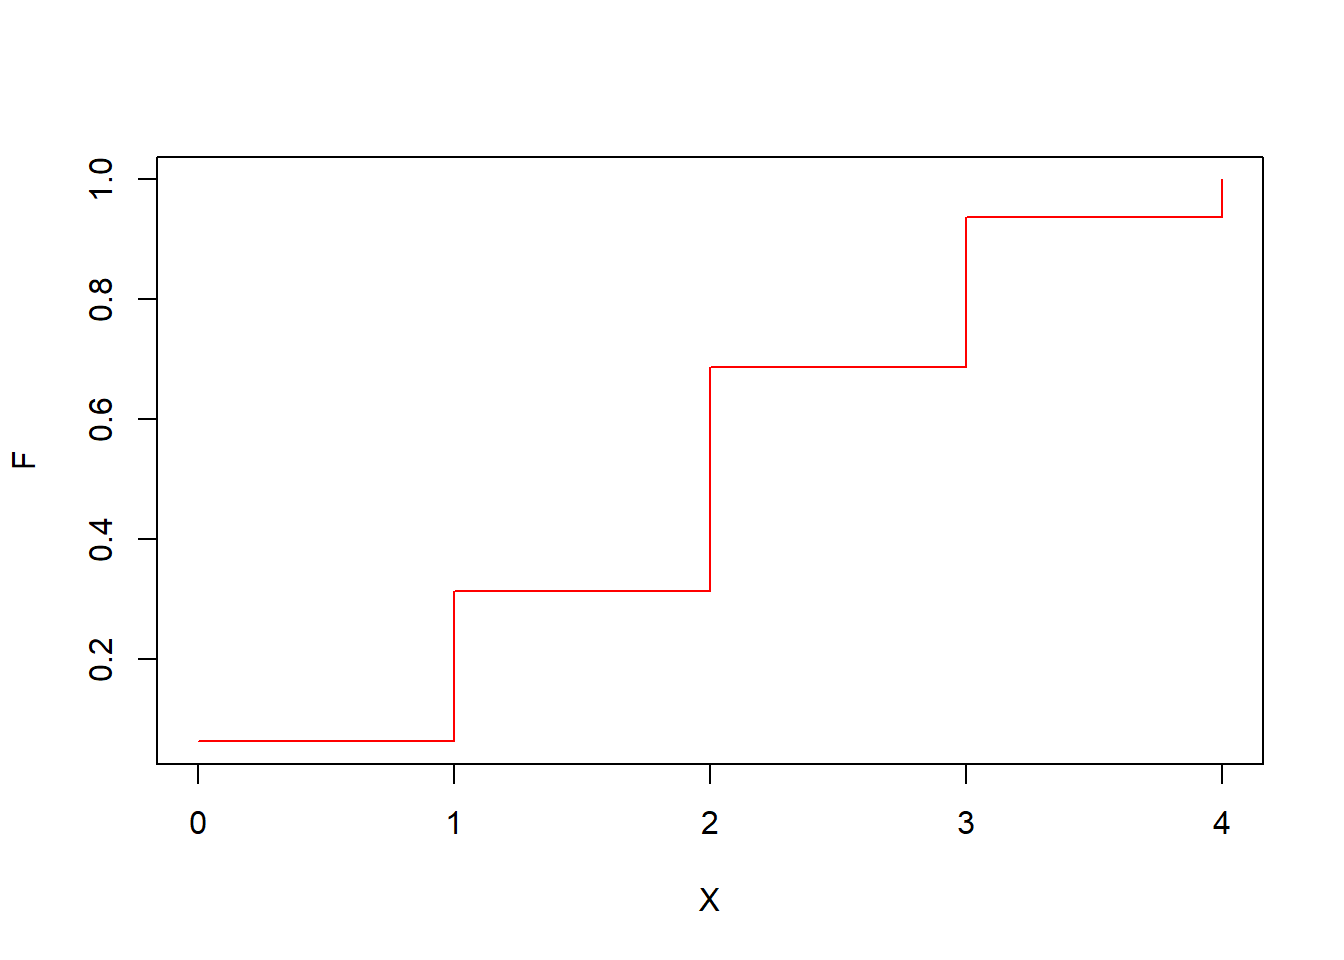
\includegraphics{_main_files/figure-latex/unnamed-chunk-39-1.pdf}

\hypertarget{ejercicio-4-1}{%
\subsubsection{Ejercicio 4}\label{ejercicio-4-1}}

Para la densidad de probabilidad

\[
    f(x)= 
\begin{cases}
    \lambda e^{-\lambda x},& \text{si } 0 \leq x\\
    0,& si \, no 
\end{cases}
\]

\begin{itemize}
\tightlist
\item
  Confirmar que se trata de una densidad de probabilidad
\item
  Hallar la distribución de probabilidad \(F(a)\)
\item
  Calcular la media
\item
  Calcule la varianza usando \(E(X^2)=V(X)+E(X)^2\)
\end{itemize}

\hypertarget{ejercicio-5-1}{%
\subsubsection{Ejercicio 5}\label{ejercicio-5-1}}

Dada la distribución acumulativa de una variable aleatoria X

\[
    F(x)= 
\begin{cases}
0, & x  < -1 \\
\frac{1}{80}(17+16x-x^2),& x \in [-1,7)\\
1,& x \geq 7\\
\end{cases}
\]

calcular:

\begin{itemize}
\tightlist
\item
  \(P(X>0)\)
\item
  \(E(X)\)
\item
  \(P(X>0|X<2)\)
\end{itemize}

\hypertarget{modelos-de-probabilidad}{%
\section{Modelos de probabilidad}\label{modelos-de-probabilidad}}

\hypertarget{ejercicio-1-4}{%
\subsubsection{Ejercicio 1}\label{ejercicio-1-4}}

Un motor de búsqueda falla al recuperar información con una probabilidad de \(0.1\)

\begin{itemize}
\item
  Si nuestro sistema recibe solicitudes de búsqueda de \(50\), ¿cuál es la probabilidad de que el sistema no responda a tres de ellas?
\item
  ¿Cuál es la probabilidad de que el motor complete con éxito búsquedas de \(15\) antes de la primera falla?
\item
  Consideramos que un buscador funciona suficientemente bien cuando es capaz de encontrar información de \(10\) solicitudes por cada \(2\) fallos. ¿Cuál es la probabilidad de que en un ensayo de fiabilidad nuestro motor de búsqueda sea satisfactorio?
\end{itemize}

\hypertarget{ejercicio-2-4}{%
\subsubsection{Ejercicio 2}\label{ejercicio-2-4}}

En una población, la probabilidad de que nazca un niño es \(p=0,51\). Considere una familia de 4 hijos.

\begin{itemize}
\tightlist
\item
  ¿Cuál es la probabilidad de que una familia tenga un solo niño?
\item
  ¿Cuál es la probabilidad de que una familia tenga una sola niña?
\item
  ¿Cuál es la probabilidad de que una familia tenga solo un niño o solo una niña?
\item
  ¿Cuál es la probabilidad de que la familia tenga al menos dos niños?
\item
  ¿Cuál es el número de hijos que debe tener una familia para que la probabilidad de tener al menos una niña sea superior a 0,75?
\end{itemize}

\hypertarget{ejercicio-3-2}{%
\subsubsection{Ejercicio 3}\label{ejercicio-3-2}}

La cantidad promedio de partículas radiactivas que golpean un contador Geiger es de \(2.3\) segundos.

\begin{itemize}
\item
  ¿Cuál es la probabilidad de contar exactamente 2 partículas en un segundo?
\item
  ¿Cuál es la probabilidad de detectar exactamente \(10\) partículas en \(5\) segundos?
\item
  ¿Cuál es la probabilidad de al menos un conteo en dos segundos?
\item
  ¿Cuál es la probabilidad de tener que esperar \(2,5\) segundos después de que encendemos el detector?
\end{itemize}

\hypertarget{ejercicio-4-2}{%
\subsubsection{Ejercicio 4}\label{ejercicio-4-2}}

\begin{itemize}
\item
  ¿Cuál es la probabilidad de que la altura de un hombre sea al menos
  \(165\)cm si la media poblacional es \(175\)cm y la desviación estándar es \(10\)cm?
\item
  ¿Cuál es la probabilidad de que la altura de un hombre esté entre
  \(165\)cm y \(180\)cm.
\item
  ¿Cuál es la altura que define el \(5\%\) de los hombres más pequeños?
\end{itemize}

\hypertarget{estimadores-puntuales}{%
\section{Estimadores puntuales}\label{estimadores-puntuales}}

\hypertarget{ejercicio-1-5}{%
\subsubsection{Ejercicio 1}\label{ejercicio-1-5}}

Considere el modelo de probabilidad

\[
    f(x)= 
\begin{cases}
    1/2-a,& \text{si } x=-1 \\ 
    1/2,& \text{si } x=0\\
    a,& 1 \text{si } x=1\\ 
\end{cases}
\]

donde \(a\) es un parámetro.

Calcule la media y la varianza de la estadística: \[T=\frac{\bar{X}}{2}+\frac{1}{4}\]

donde \(\bar{X}=\frac{1}{N}\sum_{i=1}^N X_i\)

\begin{itemize}
\item
  ¿\(T\) es un estimador sesgado de \(a\)?
\item
  ¿Es \(T\) consistente? es decir, \(V(T) \rightarrow 0\) cuando \(N\rightarrow \infty\)
\end{itemize}

\hypertarget{ejercicio-2-5}{%
\subsubsection{Ejercicio 2}\label{ejercicio-2-5}}

\begin{itemize}
\tightlist
\item
  ¿Es \(\bar{X}^2=(\frac{1}{N}\sum_{i=1}^N X_i)^2\) un estimador imparcial de \(E(X)^2\)?
\end{itemize}

\hypertarget{muestreo-y-teorema-del-luxedmite-central}{%
\section{Muestreo y teorema del límite central}\label{muestreo-y-teorema-del-luxedmite-central}}

\hypertarget{ejercicio-1-6}{%
\subsubsection{Ejercicio 1}\label{ejercicio-1-6}}

Un modelo de batería carga hasta \(75\%\) de su capacidad en una hora con una desviación estándar de \(15\%\).

\begin{itemize}
\item
  Si cobramos \(25\), ¿cuál es la probabilidad de que el promedio de la muestra esté a una distancia de \(5\%\) del cargo de la media?
\item
  Si cobramos \(100\), ¿cuál es esa probabilidad?
\item
  Si, en cambio, solo cargamos baterías de \(9\), ¿cuál es la carga que es superada por el promedio de la muestra con solo \(0.015\) de probabilidad?
\end{itemize}

\hypertarget{ejercicio-2-6}{%
\subsubsection{Ejercicio 2}\label{ejercicio-2-6}}

Se necesita un componente electrónico para el correcto funcionamiento de un telescopio. Necesita ser reemplazado inmediatamente cuando se desgasta.

La vida media del componente (\(\mu\)) es de \(100\) horas y su desviación estándar \(\sigma\) es de \(30\) horas.

\begin{itemize}
\item
  ¿Cuál es la probabilidad de que el promedio de la vida media de \(50\) componentes esté dentro de \(1\) hora de la vida media de un solo componente?
\item
  ¿Cuántos componentes necesitamos para que el telescopio esté operativo \(2750\) horas consecutivas con una probabilidad de \(0,95\)?
\end{itemize}

\hypertarget{ejercicio-3-3}{%
\subsubsection{Ejercicio 3}\label{ejercicio-3-3}}

Una máquina automática llena tubos de ensayo con muestras biológicas con una media de \(\mu=130\)mg y una desviación estándar de \(\sigma=5\)mg.

\begin{itemize}
\item
  para una muestra aleatoria de tamaño \(50\). ¿Cuál es la probabilidad de que
  la media muestral (promedio) está entre \(128\) y \(132\)gr?
\item
  ¿Cuál debe ser el tamaño de la muestra (\(n\)) para que la media muestral \(\bar{X}\) sea mayor a \(131\)gr con una probabilidad menor o igual a \(0.025\)?
\end{itemize}

\hypertarget{ejercicio-4-3}{%
\subsubsection{Ejercicio 4}\label{ejercicio-4-3}}

En el Caribe, parece haber un promedio de huracanes de \(6\) por año. Teniendo en cuenta que la formación de huracanes es un proceso de Poisson, los meteorólogos planean estimar el tiempo medio entre la formación de dos huracanes. Planean recolectar una muestra de tamaño \(36\) para los tiempos entre dos huracanes.

\begin{itemize}
\item
  ¿Cuál es la probabilidad de que su promedio muestral esté entre \(45\) y \(60\) días?
\item
  ¿Cuál debe ser el tamaño de la muestra para que tengan una probabilidad de \(0.025\) de que la media muestral sea mayor a \(70\) días?
\end{itemize}

\hypertarget{ejercicio-5-2}{%
\subsubsection{Ejercicio 5}\label{ejercicio-5-2}}

La probabilidad de que se encuentre una mutación particular en la población es de \(0.4\). Si probamos \(2000\) personas para la mutación:

\begin{itemize}
\tightlist
\item
  ¿Cuál es la probabilidad de que el número total de personas con la mutación esté entre \(791\) y \(809\)?
\end{itemize}

sugerencia: use el CLT con una muestra de ensayos de Bernoulli de \(2000\). Esto se conoce como la aproximación normal de la distribución binomial.

\hypertarget{muxe1xima-verosimilitud}{%
\section{Máxima verosimilitud}\label{muxe1xima-verosimilitud}}

\hypertarget{ejercicio-1-7}{%
\subsubsection{Ejercicio 1}\label{ejercicio-1-7}}

Para una variable aleatoria con una función de probabilidad binomial

\[f(x; p)=\binom n x p^x(1-p)^{n-x}\]

\begin{itemize}
\item
  ¿Cuál es el estimador de máxima verosimilitud de \(p\) para una muestra de tamaño \(1\) de esta variable aleatoria?
\item
  En \textbf{un} examen de \(100\) estudiantes observamos \(x_1=68\) estudiantes que aprobaron el examen. ¿Cuál es la estimación de \(p\)?
\end{itemize}

\hypertarget{ejercicio-2-7}{%
\subsubsection{Ejercicio 2}\label{ejercicio-2-7}}

Tome una variable aleatoria con la siguiente función de densidad de probabilidad

\[
f(x)=
\begin{cases}
    (1+\theta)x^\theta,& \text{si } x\in (0,1)\\
    0,&  x\notin (0,1)
\end{cases}
\]

\begin{itemize}
\item
  ¿Cuál es la estimación de máxima verosimilitud para \(\theta\)?
\item
  Si tomamos una muestra de \(5\) con observaciones
  \(x_1 = 0,92; \qquad x_2 = 0,79; \qquad x_3 = 0,90; \qquad x_4 = 0,65; \qquad x_5 = 0,86\)
\end{itemize}

¿Cuál es el valor estimado del parámetro \(\theta\)?

\hypertarget{ejercicio-3-4}{%
\subsubsection{Ejercicio 3}\label{ejercicio-3-4}}

Tome una variable aleatoria con la siguiente función de densidad de probabilidad

\[
    f(x)= 
\begin{cases}
    \lambda e^{-\lambda x},& \text{si } 0 \leq x\\
    0,& si \, no 
\end{cases}
\]

\begin{itemize}
\item
  ¿Cuál es la estimación de máxima verosimilitud para \(\lambda\)?
\item
  Si tomamos una muestra de \(5\) con observaciones
  \(x_1 = 0.223 \qquad x_2 = 0.681; \qquad x_3 = 0,117; \qquad x_4 = 0,150; \qquad x_5 = 0.520\)
\end{itemize}

¿Cuál es el valor estimado del parámetro \(\lambda\)?

\hypertarget{muxe9todo-de-los-momentos}{%
\section{Método de los momentos}\label{muxe9todo-de-los-momentos}}

\hypertarget{ejercicio-1-8}{%
\subsubsection{Ejercicio 1}\label{ejercicio-1-8}}

¿Cuáles son los estimadores de los siguientes modelos paramétricos dados por el método de los momentos?

\begin{longtable}[]{@{}lll@{}}
\toprule
modelo & f(x) & E(X) \\
\midrule
\endhead
Bernoulli & \(p^x(1-p)^{1-x}\) & \(p\) \\
binomial & \(\binom n x p^x(1-p)^{n-x}\) & \(np\) \\
Geométrico desplazado & \(p(1-p)^{x-1}\) & \(\frac{1}{p}\) \\
Binomial negativo & \(\binom {x+r-1} x p^r(1-p)^x\) & \(r\frac{1-p}{p}\) \\
Veneno & \(\frac{e^{-\lambda}\lambda^x}{x!}\) & \(\lambda\) \\
Exponencial & \(\lambda e^{-\lambda x}\) & \(\frac{1}{\lambda}\) \\
normales & \(\frac{1}{\sqrt{2\pi}\sigma}e^{-\frac{(x-\mu)^2}{2\sigma^2}}\) & \(\mu\) \\
\bottomrule
\end{longtable}

\hypertarget{ejercicio-2-8}{%
\subsubsection{Ejercicio 2}\label{ejercicio-2-8}}

Tome una variable aleatoria con la siguiente función de densidad de probabilidad

\[
f(x)=
\begin{cases}
    (1+\theta)x^\theta,& \text{si } x\in (0,1)\\
    0,& x\notin (0,1)
\end{cases}
\]

\begin{itemize}
\tightlist
\item
  Calcule \(E(X)\) como una función de \(\theta\)
\item
  ¿Cuál es la estimación de \(\theta\) utilizando el método de los momentos?
\item
  Si tomamos una muestra de \(5\) con observaciones
  \(x_1 = 0,92; \qquad x_2 = 0,79; \qquad x_3 = 0,90; \qquad x_4 = 0,65; \qquad x_5 = 0,86\)
\end{itemize}

¿Cuál es el valor estimado del parámetro \(\theta\)?

\hypertarget{ejercicio-3-5}{%
\subsubsection{Ejercicio 3}\label{ejercicio-3-5}}

Considere una variable aleatoria discreta \(X\) que sigue una distribución binomial negativa con función de masa de probabilidad:

\[f(x) = \binom{x+r-1}{x}p^r(1-p)^x\]

Dado que

\begin{itemize}
\tightlist
\item
  \(E(X)=\dfrac{r(1-p)}{p}\)
\item
  \(V(X) =\dfrac{r(1-p)}{p^2}\)
\end{itemize}

calcular:

\begin{itemize}
\item
  Una estimación del parámetro \(r\) y una estimación del parámetro \(p\) obtenidas a partir de una muestra aleatoria de tamaño \(n\) por el método de los momentos.
\item
  Los valores de las estimaciones de \(r\) y \(p\) para la siguiente muestra aleatoria:
\end{itemize}

\[x_1 = 27; \qquad x_2 = 8; \qquad x_3 = 22; \qquad x_4 = 29; \qquad x_5 = 19; \qquad x_5 = 32\]

  \bibliography{book.bib,packages.bib}

\end{document}
